% Author: Chenyang Zhang
% License: LaTeX Project Public License v1.3c
% 完整编译: XeLaTex -> BibTex -> XeLaTex -> XeLaTex
% GitHub项目地址:https://github.com/zcyeee/HNU_LaTeX_Template

%%%%%%%%%%%%%%%%%%%%%%%%  文档配置  %%%%%%%%%%%%%%%%%%%%%%%%

\documentclass[
    report,     % 文档类型
    oneside,    % 单双栏
    UTF8,       % 字符集
    zihao=-4    % 全局字号(-4是小四号的意思)
]{config} % 配置文件模板 config.cls


% 封面图片定义
\def \titlePageImages{
    
\includegraphics[width=0.23\textwidth] {figures/logos/ruc_logo.eps}\\ % 湖南大学校徽
    \vspace{10pt}
    
\includegraphics[width=0.5\textwidth] {figures/logos/ruc_text.eps}\\ % 湖南大学校名
}

\vspace{10pt}

% 文档信息定义
\def \majorTitle   {人工智能与Python程序设计} % 大标题
\def \minorTitleCN {Group 1 模型审计报告} % 中文标题
\def \minorTitleEN {Model Validation Report - Group 1} % 英文标题

% 个人信息定义
\def \titlePageInfoBox{
    % 参数:#1下划线长度 #2字号 #3标题 #4内容
    \infobox{6.00cm}{0.65cm}{所在学院}{财政金融学院}\\
    \infobox{6.00cm}{0.65cm}{组~~~~~~~~别}{Group 1}\\
    \infobox{6.00cm}{0.65cm}{成~~~~员~~1}{崔天佑}\\
    \infobox{6.00cm}{0.65cm}{成~~~~员~~2}{席书漫}\\
    \infobox{6.00cm}{0.65cm}{成~~~~员~~3}{王晨曦}\\
    \infobox{6.00cm}{0.65cm}{成~~~~员~~4}{王瑜琪}\\

    \vspace{1cm}
}

\def \currentDate{
    2024年11月21日
}


% 设置行间距为1.5倍
\linespread{1.5}

%%%%%%%%%%%%%%%%%%%%%%%%  文档开始  %%%%%%%%%%%%%%%%%%%%%%%%

\begin{document}

% 封面
\CoverPage
    {right} % 封面类型:both、left、right、empty
    {1.000cm} % 大标题字号大小
    {0.825cm} % 中文标题字号大小
    {0.800cm} % 英文标题字号大小

%%%%%%%%%%%%%%%%%%%%%  正文前页眉页脚  %%%%%%%%%%%%%%%%%%%%%%

% 页眉(关闭页眉务必将页眉类型设为empty)
\Header
    {common} % 页眉类型:common、publish、empty
    {1pt} % 上分隔线宽度
    {1pt} % 两线距离
    {0.5pt} % 下分割线宽度
    {} % 页眉左自定义内容(文本或图片)
    % {
\includegraphics[width=0.25\textwidth]{figures/logos/school_sf_logo.jpg}} % 页眉中自定义内容(文本或图片)
    {\minorTitleCN}
    {} % 页眉右自定义内容(文本或图片)

%============================================%

% 页脚(关闭页脚务必将页脚类型设为empty) 
\Footer
    {common} % 页脚类型:common、publish、empty
    {0pt} % 上分隔线宽度
    {0pt} % 两线距离
    {0pt} % 下分割线宽度
    {} % 页脚左自定义内容(文本或图片)
    {\thepage} % 页脚中自定义内容(文本或图片)
    {} % 页脚右自定义内容(文本或图片)

%============================================%

% 页数样式 参数:#1起始页数
\SetRomanPageNumber{} % 设置罗马数字页码
% \SetArabicPageNumber{} % 设置阿拉伯数字页码
\ResetCounter{1} % 重置页数

%%%%%%%%%%%%%%%%%%%%%%%%  摘要  %%%%%%%%%%%%%%%%%%%%%%%

\begin{abstractCN}[0.6cm] % 中文摘要,参数:#1中文摘要标题字号

在当今以数据为核心的商业时代,模型审计的作用变得尤为关键,它不仅保障了决策的科学性和业务流程的高效性,
还有效降低了潜在风险。本报告由第 1 组编制,旨在深入审计第 2 组所开发的房地产估值模型。
通过细致审查第 2 组的代码,我们全面回顾了从数据清洗到模型训练和预测的每个环节,并提取了模型训练中的关键数据,
通过可视化手段提升了模型的透明度。本报告深入分析了第 2 组在数据清洗阶段的数据质量问题,并提出了改进数据清洗过程的策略。
此外,通过对 OLS、Lasso、Ridge 和 ElasticNet 四种模型的性能对比,我们探讨了它们在房地产估值中的适用性,
并为模型优化提出了具体建议。
我们期望本报告能激发双方的交流与合作,优势互补,彼此促进对Python课程的学习,互相学习,共同进步!
    
% 中文关键词
\def\keywordsCN{模型审计;线性模型;房地产估值;机器学习}

\end{abstractCN}

%============================================%

\begin{abstractEN}[0.6cm] % 英文摘要,参数:#1英文摘要标题字号

In today's data-centric business era, the role of model auditing has become particularly critical, 
not only to ensure scientific decision-making and efficient business processes, but also to mitigate potential risks. 
This report has been carefully prepared by Group 1 to provide an in-depth audit of the real estate valuation model developed by Group 2. 
By scrutinizing the code of Group 2, we comprehensively reviewed each step from data cleansing to model training and prediction, 
and extracted the key data in model training to enhance the transparency of the model through visualization. 
This report analyzes in depth the data quality problems of Group 2 in the data cleaning stage and proposes strategies to improve the data cleaning process. 
In addition, by comparing the performance of four models - OLS, Lasso, Ridge, and ElasticNet - we explore their applicability in real estate valuation and make specific suggestions for model optimization. 
We expect that this report will stimulate communication and co-operation, complement each other's strengths, promote each other's learning of Python courses, and learn from each other to make progress together!

% 英文关键词
\def\keywordsEN{Model validation; Linear models; Real estate valuation; Machine learning}

\end{abstractEN}

%%%%%%%%%%%%%%%%%%%%%%%%  启用目录  %%%%%%%%%%%%%%%%%%%%%%%%

% 目录,参数: 
% #1目录类型:next(分页显示)、current(同页显示)
% #2目录行距
% #3目录标题
% #4当前章节名
\contentPage{next}{1.5}{目~~~~录}{目录}
\vspace{13pt}
\contentpageOfFigures{next}{1.5}{图目录}{图目录}
\vspace{20pt}
\contentpageOfTables{current}{1.5}{表目录}{表目录}

%%%%%%%%%%%%%%%%%%%%%%%%  启用水印  %%%%%%%%%%%%%%%%%%%%%%%%

% 若正文不需要水印把这部分命令删掉就好
\imageWatermark % 图片水印
    {0} % 旋转角度
    {0.7} % 放缩倍率
    {0.03} % 透明度 0-1
    {figures/logos/ruc_logo.eps} % 图片路径

%%%%%%%%%%%%%%%%%%%%%%  正文页眉页脚  %%%%%%%%%%%%%%%%%%%%%%%

% 页眉(关闭页眉务必将页眉类型设为empty)
\Header
    {common} % 页眉类型:common、publish、empty
    {1pt} % 上分隔线宽度
    {1pt} % 两线距离
    {0.5pt} % 下分割线宽度
    {\minorTitleCN} % 页眉左自定义内容(文本或图片)
    {} % 页眉中自定义内容(文本或图片)}
    {\currentChapterInfo} % 页眉右自定义内容(文本或图片)

%============================================%

% 页脚(关闭页脚务必将页脚类型设为empty) 
\Footer
    {common} % 页脚类型:common、publish、empty
    {0pt} % 上分隔线宽度
    {0pt} % 两线距离
    {0pt} % 下分割线宽度
    {} % 页脚左自定义内容(文本或图片)
    {\thepage} % 页脚中自定义内容(文本或图片)
    {} % 页脚右自定义内容(文本或图片)

%============================================%

% 页数样式 参数:#1起始页数
% \SetRomanPageNumber{} % 设置罗马数字页码
\SetArabicPageNumber{} % 设置阿拉伯数字页码
\ResetCounter{1} % 重置页数

%%%%%%%%%%%%%%%%%%%%%%%%%  正文  %%%%%%%%%%%%%%%%%%%%%%%%%%
% 代码插入示例
% \begin{lstlisting}[label=code:ols_features, language=Python, caption=OLS模型特征选取]

% \end{lstlisting}

\chapter{引言}

在当今数据驱动的时代,模型优化与验证(Model Validation)不仅是数据分析流程中不可或缺的一环,更是确保决策科学性、提升业务效率与降低潜在风险的基石。模型,作为连接数据与决策的桥梁,其准确性、稳定性和可靠性直接关系到企业战略部署的成功与否。因此,深入实施模型验证,不仅是对数据科学严谨态度的体现,更是对企业未来发展的负责。

模型验证的核心价值在于,它为我们提供了一套系统化、标准化的方法,用以评估模型在实际应用场景中的表现。这一过程不仅包括对模型预测能力的验证,即模型能否准确反映数据间的内在规律;还涵盖了模型的稳健性测试,即面对数据波动或异常值时,模型是否能保持稳定的性能输出。通过这一系列严格而细致的校验,我们能够及时发现并修正模型设计中的潜在缺陷,避免“trash in, trash out”的恶性循环,确保最终输出的预测结果或决策建议具备高度的可信度。

此外,模型验证还有助于提升业务决策的透明度和可追溯性。在高度监管的行业环境中,能够清晰展示模型验证的过程与结果,是赢得内外部信任的关键。它让决策者理解模型背后的逻辑与假设,从而更加自信地依据模型输出做出判断。同时,当模型预测结果与实际情况出现偏差时,完善的验证机制能够帮助我们迅速定位问题源头,无论是数据质量问题、模型假设不当还是算法本身的局限性,都能得到及时有效的反馈与调整。

总而言之,模型验证是连接理论模型与实践应用的纽带,它不仅是提升模型性能、优化预测精度的技术手段,更是构建数据驱动文化、增强企业竞争力的战略选择。通过持续不断地对模型进行验证与优化,我们能够更好地驾驭数据的力量,为决策提供坚实的数据支撑,助力企业在复杂多变的市场环境中稳健前行。因此,本次报告在学习研究第2组同学代码的基础上,探讨性提出一系列模型优化的建议,旨在通过这一交流过程,促进双方在相互学习与良性竞争中共同进步。

\chapter{数据清洗}
\section{定性数据}
\subsection{部分特征集中处理}

\textbf{(1) 导入数据}

通过循环将列(\lstinline|'区域'|、\lstinline|'板块'|、\lstinline|'城市'|、\lstinline|'交易权属'|、
\lstinline|'房屋用途'|、\lstinline|'产权所属'|)
从原始数据集复制到清洗后的数据集中。这些列没有缺失值。

\textbf{(2) 补充部分列的缺失值}

定义函数\lstinline|fill_missing_values|,将列(\lstinline|'建筑结构'|、\lstinline|'装修情况'|、\lstinline|'别墅类型'|)
中的缺失值填补为字符串\lstinline|'未知'|,填补后的列复制到清洗后的数据框中。

\subsection{环线的处理}
\textbf{(1) 构建BallTree}

代码先将经纬度从度数转换为弧度,以便使用\lstinline|BallTree|进行基于地理位置的最近邻搜索。
然后使用训练集中有环线信息的数据构建\lstinline|BallTree|,
并使用\lstinline|haversine|距离度量,它适用于球面上的距离计算。

\lstinline|BallTree|是一种用于多维空间数据索引和查询的数据结构,
它基于球体层次结构(即“球树”)构建,常用于高效地执行最近邻搜索。
在机器学习和数据科学中,\lstinline|BallTree|可以用于快速找到给定点的最近邻点,
这在许多应用中非常有用,比如聚类、分类、回归和密度估计。
\lstinline|BallTree|的工作原理基于分而治之的策略。它将空间递归地划分成一系列的球体,
每个球体代表一个节点。在构建\lstinline|BallTree|时,算法会选择一个点作为中心,
然后找到包含所有点的最小球体,这个球体就是根节点。接着,
算法会递归地对球体内的点集进行同样的操作,直到所有的点都被包含在树的叶节点中。

\textbf{(2) 处理缺失值}

定义函数\lstinline|fill_missing_ring_using_balltree|,接受一行数据、包含环线信息的数据集、
以及构建好的\lstinline|BallTree|作为参数。如果当前行已经有环线数据,
则直接返回该值;如果没有,则使用\lstinline|BallTree|找到最近的有环线信息的地点,并返回其环线值。

\textbf{(3) 方法优势}

在精确度方面,该方法假设地理位置相近的点具有相似的特征,利用这种相关性有效地填补“环线”缺失值。
在计算效率上,\lstinline|BallTree|的最近邻搜索方法,尤其是在高维空间中,使得填补大量数据的缺失值变得高效。

\newpage

\begin{lstlisting}[label=code:ring_processing, language=Python, caption=环线处理]
    # 1. 先将经纬度转换为弧度,以便于使用BallTree
    X_train['lat_rad'] = np.radians(X_train['lat'])
    X_train['lon_rad'] = np.radians(X_train['lon'])
    
    X_test['lat_rad'] = np.radians(X_test['lat'])
    X_test['lon_rad'] = np.radians(X_test['lon'])
    
    X_predict['lat_rad'] = np.radians(X_predict['lat'])
    X_predict['lon_rad'] = np.radians(X_predict['lon'])
    
    # 2. 使用训练集中有环线信息的数据构建BallTree
    train_with_ring = X_train[X_train['环线'].notnull()].copy()
    coords_train_with_ring = np.vstack((train_with_ring['lat_rad'], train_with_ring['lon_rad'])).T
    tree_train_with_ring = BallTree(coords_train_with_ring, metric='haversine')
    
    # 3. 创建辅助函数,用于填补缺失的环线数据
    def fill_missing_ring_using_balltree(row, df_with_ring, tree_with_ring, lat_col='lat', lon_col='lon', ring_col='环线'):
        # 如果当前行有环线数据,直接返回原值
        if pd.notnull(row[ring_col]):
            return row[ring_col]
        
        # 当前行的经纬度(转换为弧度)
        current_location_rad = np.radians([row[lat_col], row[lon_col]]).reshape(1, -1)
        
        # 查找最近的小区,限定在有环线数据的小区范围内
        dist, idx = tree_with_ring.query(current_location_rad, k=1)  # 只找一个最近的小区
        nearest_idx = idx[0][0]  # 取出最近小区的索引
        
        # 返回最近小区的环线值
        return df_with_ring.iloc[nearest_idx][ring_col]
    
    # 4. 填补训练集中的缺失值(使用训练集内的最近邻小区数据填补)
    X_train_cleaned['环线'] = X_train.apply(
        lambda row: fill_missing_ring_using_balltree(row, train_with_ring, tree_train_with_ring), axis=1
    )
    
    # 5. 填补测试集中的缺失值(使用训练集中的最近邻小区数据填补)
    X_test_cleaned['环线'] = X_test.apply(
        lambda row: fill_missing_ring_using_balltree(row, train_with_ring, tree_train_with_ring), axis=1
    )
    
    X_predict_cleaned['环线'] = X_predict.apply(
        lambda row: fill_missing_ring_using_balltree(row, train_with_ring, tree_train_with_ring), axis=1
    )
    
    # 6. 删除临时添加的经纬度弧度列(lat_rad 和 lon_rad)
    X_train.drop(columns=['lat_rad', 'lon_rad'], inplace=True)
    X_test.drop(columns=['lat_rad', 'lon_rad'], inplace=True)
    
    # 查看处理后的结果
    print(X_train_cleaned[['环线']].head())
    print(X_test_cleaned[['环线']].head())
\end{lstlisting}

\subsection{配备电梯的处理}
\textbf{(1) 消除链式赋值的警告}

\lstinline|pd.options.mode.chained_assignment = None|这行代码用于关闭lstinline|Pandas|在进行链式赋值时产生的警告。
链式赋值是指像\lstinline|df['A']['B'] = value|这样的操作,
其中\lstinline|df['A']['B']|返回的是一个 Series,直接赋值可能会导致\lstinline|SettingWithCopyWarning|警告。

\textbf{(2) 处理缺失值}

\lstinline|process_elevator|函数使用\lstinline|.notna()|
方法检查“梯户比例”列中的值是否非空,使用\lstinline|.map()|方法将
True/False值映射为 '有'/'无',表示是否配备电梯。
再调用\lstinline|fill_missing_values|函数填补“配备电梯”列中的缺失值,填补值为 '无'。

\textbf{(3) 可能存在的问题}
\begin{itemize}
    \item 这部分并没有链式赋值的操作,代码赘余。
    \item 关联逻辑赘余,可直接将“配备电梯”列中的缺失值填补为“无”。
\end{itemize}

下面的代码\ref{code:elevator_processing}展示了配备电梯特征的处理过程。
\begin{lstlisting}[label=code:elevator_processing, language=Python, caption=配备电梯的处理代码]
    # 消除链式赋值的警告
    pd.options.mode.chained_assignment = None
    
    # 处理“配备电梯”列:根据“梯户比例”判断
    def process_elevator(df, df_cleaned, elevator_col, ratio_col):
        # 根据“梯户比例”列是否有值判断是否配备电梯
        df[elevator_col] = df[ratio_col].notna().map({True: '有', False: '无'})
        fill_missing_values(df, df_cleaned, elevator_col, '无')
    
    # 应用“配备电梯”列的处理函数
    process_elevator(X_train, X_train_cleaned, '配备电梯', '梯户比例')
    process_elevator(X_test, X_test_cleaned, '配备电梯', '梯户比例')
    process_elevator(X_predict, X_predict_cleaned, '配备电梯', '梯户比例')
\end{lstlisting}

\subsection{房屋朝向和房屋优势的处理}

\textbf{(1) 房屋朝向的处理}

定义标准方向和映射规则:\lstinline|standard_directions|定义八个标准方向,
\lstinline|direction_mapping|定义映射规则
,将非标准的方向(如“南东”)映射到标准方向(如“东南”)。

定义处理函数\lstinline|clean_directions_optimized|,使用\lstinline|str.split()|方法将房屋朝向字符串分割成单独的方向词。
通过循环\lstinline|direction_mapping|中的映射规则,将非标准方向替换为标准方向。
使用\lstinline|MultiLabelBinarizer|将方向列表转换为布尔特征,即每个方向都作为一个特征,如果列表中包含该方向,则对应的特征值为True,否则为False。

\textbf{(2) 房屋优势的处理}

定义处理函数\lstinline|process_advantages_optimized|,使用\lstinline|fillna('')|
将缺失值替换为空字符串,然后使用\lstinline|str.split('、')|方法按顿号分割房屋优势字符串,使用\lstinline|MultiLabelBinarizer|,将每个房屋的优势列表转化为布尔矩阵。

\textbf{(3) 可能存在的问题}

\begin{itemize}
    \item 将文本特征转换为布尔特征可能会丢失一些信息,例如文本中的数量或强度等。在房屋朝向的处理中,布尔特征只保留了方向的有无,没有考虑方向的强度或权重。
    \item 单纯的布尔特征可能无法表达特征间的组合关系,例如“东南”和“东”同时出现可能表示一个特定的区域,但单独的布尔特征无法表达这种组合关系。
    \item 如果特征很多,转换后的布尔特征空间可能会非常大,导致维度灾难,增加模型训练的难度和计算成本,且容易增加模型过度拟合的风险,尤其是在样本量不足的情况下。
\end{itemize}

下面的代码\ref{code:bool_features}展示了配备房屋朝向和房屋优势的处理过程。
\begin{lstlisting}[label=code:bool_features, language=Python, caption=房屋朝向和房屋优势的处理代码]
    # 定义标准的八个方向
    standard_directions = ['东', '南', '西', '北', '东南', '东北', '西南', '西北']
    
    # 定义一个方向映射规则,将“南东”标准化为“东南”
    direction_mapping = {
        '南东': '东南',
        '北东': '东北',
        '南西': '西南',
        '北西': '西北',
        '东南': '东南',
        '东北': '东北',
        '西南': '西南',
        '西北': '西北'
    }
    
    # 优化房屋朝向处理
    def clean_directions_optimized(series):
        # 用空格分割各个方向
        direction_split = series.str.split()
        
        # 通过替换将“南东”等非标准化的方向转换为标准方向
        for key, value in direction_mapping.items():
            direction_split = direction_split.apply(lambda x: [value if d == key else d for d in x])
        
        # 将方向列表去重,并通过 MultiLabelBinarizer 生成布尔特征
        mlb = MultiLabelBinarizer(classes=standard_directions)
        return pd.DataFrame(mlb.fit_transform(direction_split), columns=mlb.classes_, index=series.index)
    
    # 应用优化后的函数到房屋朝向列,并将结果添加
    X_train_cleaned = pd.concat([X_train_cleaned, clean_directions_optimized(X_train['房屋朝向'])], axis=1)
    X_test_cleaned = pd.concat([X_test_cleaned, clean_directions_optimized(X_test['房屋朝向'])], axis=1)
    X_predict_cleaned = pd.concat([X_predict_cleaned, clean_directions_optimized(X_predict['房屋朝向'])], axis=1)
    
    # 优化房屋优势处理,去除空白字符
    def process_advantages_optimized(series):
        # 按“、”分割房屋优势,去除空格和空字符串
        advantage_split = series.fillna('').apply(lambda x: [item.strip() for item in x.split('、') if item.strip()])
        
        # 通过 MultiLabelBinarizer 生成布尔特征
        mlb = MultiLabelBinarizer()
        return pd.DataFrame(mlb.fit_transform(advantage_split), columns=mlb.classes_, index=series.index)
    
    # 应用优化后的函数到房屋优势列,并将结果添加
    X_train_cleaned = pd.concat([X_train_cleaned, process_advantages_optimized(X_train['房屋优势'])], axis=1)
    X_test_cleaned = pd.concat([X_test_cleaned, process_advantages_optimized(X_test['房屋优势'])], axis=1)
    X_predict_cleaned = pd.concat([X_predict_cleaned, process_advantages_optimized(X_predict['房屋优势'])], axis=1)
    
    # 查看处理后的数据框
    print(X_train_cleaned.head())
    print(X_test_cleaned.head())
\end{lstlisting}

\subsection{房屋年限的处理}
\textbf{(1) 代码解释}

\lstinline|process_house_age|函数使用\lstinline|if-elif-else|结构来判断\lstinline|age_info|的值,并返回对应的数值: '满五年'返回 5,'满两年'返回 2, '未满两年'返回 0,其他值(包括缺失值)返回\lstinline|None|。

使用\lstinline|fillna|方法,用训练集中位数填补训练集 “房屋年限” 列中的缺失值。

\textbf{(2) 可能存在的问题}

\begin{itemize}
    \item 中位数填充可能会影响数据的分布,尤其是在数据偏斜的情况下。如果数据集中存在极端值,中位数可能是一个比平均值更好的中心趋势度量,但如果数据分布接近对称,使用中位数可能会引入偏差。如果数据是随机的,中位数填充可能引起偏差。
    \item 将“满两年”映射为2,“满五年”映射为5,可能会让人误以为这些数值代表具体的年数,从而在数据分析和模型解释时产生误解。且直接使用数值2和5可能会影响数据的整体分布,特别是在进行数值运算或数据标准化时。
\end{itemize}

下面的代码\ref{code:house_age}展示了房屋年限的处理过程。

\newpage
\begin{lstlisting}[label=code:house_age, language=Python, caption=房屋年限的处理代码]
    # 1. 定义处理“房屋年限”的函数
    def process_house_age(age_info):
        if age_info == '满五年':
            return 5
        elif age_info == '满两年':
            return 2
        elif age_info == '未满两年':
            return 0
        else:
            return None  # 如果是缺失值或不匹配,返回 None
    
    # 2. 处理训练集的“房屋年限”列
    X_train_cleaned['房屋年限'] = X_train['房屋年限'].apply(process_house_age)
    
    # 3. 计算训练集中“房屋年限”的中位数(用于填补缺失值)
    train_median_age = X_train_cleaned['房屋年限'].median()
    
    # 4. 处理测试集的“房屋年限”列
    X_test_cleaned['房屋年限'] = X_test['房屋年限'].apply(process_house_age)
    X_predict_cleaned['房屋年限'] = X_predict['房屋年限'].apply(process_house_age)
    
    
    # 5. 填补训练集中的缺失值
    X_train_cleaned['房屋年限'] = X_train_cleaned['房屋年限'].fillna(train_median_age)
    
    # 6. 填补测试集中的缺失值,使用训练集的中位数
    X_test_cleaned['房屋年限'] = X_test_cleaned['房屋年限'].fillna(train_median_age)
    X_predict_cleaned['房屋年限'] = X_predict_cleaned['房屋年限'].fillna(train_median_age)
    
    # 查看处理后的结果
    print(X_train_cleaned.head())
    print(X_test_cleaned.head())
\end{lstlisting}

\subsection{Word2Vec处理长文本数据}

\textbf{(1) 代码解释}

将(\lstinline|核心卖点|, \lstinline|户型介绍|, \lstinline|周边配套|, \lstinline|交通出行|)每列文本分割为单词列表,基于训练集语料库训练一个\textbf{Word2Vec}模型,将每段文本表示为单词词向量的平均值,并拆分为100维特征向量添加到数据集中。

Word2Vec是一种用于生成词嵌入(word embeddings)的模型,它通过学习文本语料库中的单词的上下文关系来生成每个单词的数值向量表示。Word2Vec模型的核心思想是:在文本中经常一起出现的单词在向量空间中也会彼此接近,从而进行语义捕捉。

\textbf{(2) 可能存在的问题}

\begin{itemize}
    \item 仅基于训练集训练的Word2Vec模型可能无法很好地泛化到测试集和预测集。
    \item 最终得出的变量个数过多,会导致模型复杂性提升,浪费计算资源。
\end{itemize}

下面的代码\ref{code:house_age}展示了利用Word2Vec处理长文本数据的处理过程。
\begin{lstlisting}[label=code:word2vec, language=Python, caption=Word2Vec处理长文本数据的处理代码]
    # 处理缺失值,确保所有数据为字符串类型
    for col in ['核心卖点', '户型介绍', '周边配套', '交通出行']:
        X_train[col] = X_train[col].fillna('未知').astype(str)
        X_test[col] = X_test[col].fillna('未知').astype(str)
        X_predict[col] = X_predict[col].fillna('未知').astype(str)
    
    # 定义文本清理函数
    def clean_text(text):
        text = re.sub(r'[^\w\s]', '', text)  # 去除标点符号
        text = text.lower()  # 转为小写
        return text
    
    # 应用文本清理函数
    for col in ['核心卖点', '户型介绍', '周边配套', '交通出行']:
        X_train[col] = X_train[col].apply(clean_text)
        X_test[col] = X_test[col].apply(clean_text)
        X_predict[col] = X_predict[col].apply(clean_text)
    
    # 将文本列转换为单词列表
    for col in ['核心卖点', '户型介绍', '周边配套', '交通出行']:
        X_train[col] = X_train[col].apply(lambda x: x.split())
        X_test[col] = X_test[col].apply(lambda x: x.split())
        X_predict[col] = X_predict[col].apply(lambda x: x.split())
    
    # 合并训练集所有列,创建训练语料库
    sentences_train = X_train['核心卖点'].tolist() + X_train['户型介绍'].tolist() + X_train['周边配套'].tolist() + X_train['交通出行'].tolist()
    
    # 训练Word2Vec模型(仅基于训练集)
    w2v_model = Word2Vec(sentences_train, vector_size=100, window=5, min_count=1, workers=4)
    
    # 保存Word2Vec模型
    w2v_model.save("word2vec_model.model")
    
    # 载入模型以验证保存是否成功
    w2v_model = Word2Vec.load("word2vec_model.model")
    
    # 获取训练好的词向量
    word_vectors = w2v_model.wv
    
    # 定义函数,将文本行转化为词向量的平均值
    def get_average_word2vec(text, model, vector_size):
        feature_vector = np.zeros((vector_size,), dtype='float32')
        num_words = 0
        for word in text:
            if word in model:
                num_words += 1
                feature_vector = np.add(feature_vector, model[word])
        if num_words > 0:
            feature_vector = np.divide(feature_vector, num_words)
        return feature_vector.tolist()  # 将NumPy数组转换为Python列表
    
    # 为训练集和测试集每个列生成词向量特征
    X_train_backup = X_train.copy()  # 确保有数据副本
    X_test_backup = X_test.copy()
    X_predict_backup = X_predict.copy()
    
    for col in ['核心卖点', '户型介绍', '周边配套', '交通出行']:
        X_train_backup[f'{col}_word2vec'] = X_train[col].apply(lambda x: get_average_word2vec(x, word_vectors, 100))
        X_test_backup[f'{col}_word2vec'] = X_test[col].apply(lambda x: get_average_word2vec(x, word_vectors, 100))
        X_predict_backup[f'{col}_word2vec'] = X_predict[col].apply(lambda x: get_average_word2vec(x, word_vectors, 100))
    
    # 拆分嵌入向量为独立的列
    word2vec_features = ['核心卖点_word2vec', '户型介绍_word2vec', '周边配套_word2vec', '交通出行_word2vec']
    
    for feature in word2vec_features:
        # 对训练集进行处理
        vectors_train = pd.DataFrame(X_train_backup[feature].tolist(), index=X_train_backup.index)
        vectors_train.columns = [f'{feature}_{i}' for i in range(100)]  # 命名每个列
        X_train_cleaned = pd.concat([X_train_cleaned, vectors_train], axis=1)
        
        # 对测试集进行处理
        vectors_test = pd.DataFrame(X_test_backup[feature].tolist(), index=X_test_backup.index)
        vectors_test.columns = [f'{feature}_{i}' for i in range(100)]  # 命名每个列
        X_test_cleaned = pd.concat([X_test_cleaned, vectors_test], axis=1)
    
        vectors_predict = pd.DataFrame(X_predict_backup[feature].tolist(), index=X_predict_backup.index)
        vectors_predict.columns = [f'{feature}_{i}' for i in range(100)]  # 命名每个列
        X_predict_cleaned = pd.concat([X_predict_cleaned, vectors_predict], axis=1)
    
    
    # 查看清洗后的数据
    print(X_train_cleaned.head())
    print(X_test_cleaned.head())
\end{lstlisting}

\subsection{虚拟变量化}

对指定的定性变量(\lstinline|categorical_columns|列表)逐一应用\lstinline|pd.get_dummies|,将其转化为多个二进制列(One-Hot 编码),同时使用\lstinline|drop_first=True|避免多重共线性。替换原始列为虚拟变量。

下面的代码\ref{code:virtual_variable}展示了虚拟变量化的处理过程。

\begin{lstlisting}[label=code:virtual_variable, language=Python, caption=虚拟变量化代码]
    # 定义需要虚拟变量化的定性变量
    categorical_columns = [
        '城市', '区域', '板块', '环线', '建筑结构', 
        '装修情况', '配备电梯', '别墅类型', '交易权属', '房屋用途', '产权所属'
    ]
    
    # 对训练集和测试集的指定列进行虚拟变量化,并替换原列
    for col in categorical_columns:
        # 对训练集进行虚拟变量化,并用虚拟变量替换原列
        dummies_train = pd.get_dummies(X_train_cleaned[col], prefix=col, drop_first=True)
        X_train_cleaned = pd.concat([X_train_cleaned.drop(columns=[col]), dummies_train], axis=1)
        
        # 对测试集进行虚拟变量化,并用虚拟变量替换原列
        dummies_test = pd.get_dummies(X_test_cleaned[col], prefix=col, drop_first=True)
        X_test_cleaned = pd.concat([X_test_cleaned.drop(columns=[col]), dummies_test], axis=1)
    
        dummies_predict = pd.get_dummies(X_predict_cleaned[col], prefix=col, drop_first=True)
        X_predict_cleaned = pd.concat([X_predict_cleaned.drop(columns=[col]), dummies_predict], axis=1)
    
    
    # 保证测试集和训练集列一致(如果有不匹配列,测试集中缺少的列用0填充)
    X_test_cleaned = X_test_cleaned.reindex(columns=X_train_cleaned.columns, fill_value=0)
    X_predict_cleaned = X_predict_cleaned.reindex(columns=X_train_cleaned.columns, fill_value=0)
    
    # 查看替换后的数据框结构
    print(X_train_cleaned.head())
    print(X_test_cleaned.head())
    print(X_predict_cleaned.head())
\end{lstlisting}

\section{数值型数据}

\subsection{值得借鉴和学习的点}

\textbf{(1) 交易时间的处理}

第2组的模型中使用了时间特征编码,对月度、季度等数据进行了正余弦编码以方便周期特征在模型中的使用。转化如下:
\begin{align}
    X_{\sin}&=\sin(2\pi\cdot\frac{x}{\max X}) \\
    X_{\cos}&=\cos(2\pi\cdot\frac{x}{\max X}) 
\end{align}

该过程实现如代码\ref{code:time_encoding}所示:

\begin{lstlisting}[label=code:time_encoding, language=Python, caption=交易时间的处理代码]
    def create_cyclic_features(df, column, period):
        df[f'{column}_sin'] = np.sin(2 * np.pi * df[column] / period)
        df[f'{column}_cos'] = np.cos(2 * np.pi * df[column] / period)
\end{lstlisting}

\textbf{(2) 数据标准化}

第2组的模型还对数据进行了标准化处理,代码如下所示。
\begin{lstlisting}[label=code:standardization, language=Python, caption=数据标准化代码]
    quantitative_columns = [
        'lon', 'lat', '年份', '建筑面积', '套内面积', '室', '厅', '厨', '卫',
        '楼层数值', '总层数', '梯户比例', '交易年份', '交易月份_sin', '交易月份_cos',
        '交易季度_sin', '交易季度_cos', '上次交易年份', '上次交易月份_sin',
        '上次交易月份_cos', '上次交易季度_sin', '上次交易季度_cos'
    ]
    
    # 将 word2vec 的特征列名添加到要标准化的列列表中
    for prefix in ['核心卖点_word2vec_', '户型介绍_word2vec_', '周边配套_word2vec_', '交通出行_word2vec_']:
        quantitative_columns.extend([f"{prefix}{i}" for i in range(100)])  # 假设每个 word2vec 列包含100个向量值
    
    # 初始化标准化器并拟合训练集的定量特征
    scaler = StandardScaler()
    scaler.fit(X_train_cleaned[quantitative_columns])
    
    # 对训练集和测试集进行标准化
    X_train_cleaned[quantitative_columns] = scaler.transform(X_train_cleaned[quantitative_columns])
    X_test_cleaned[quantitative_columns] = scaler.transform(X_test_cleaned[quantitative_columns])
    X_predict_cleaned[quantitative_columns] = scaler.transform(X_predict_cleaned[quantitative_columns])
\end{lstlisting}

通过标准化便利后续的模型选取。标准化后的数据才可以进行Lasso、Ridge、主成分分析等方法的回归分析。

\subsection{可能存在争议的问题}

\textbf{(1) 所在楼层的处理}

第2组选择的处理方法是:提取总楼层数,高中低各取总层数的5/6 3/6 1/6,地下室为-1。

此方法存在的一个较大问题是对不同楼层的效应人为添加了相关关系:此关系默认了高楼层的影响与中楼层或低楼层的影响存在倍数关系。然而这层倍数关系是人为臆测的,可能造成较大的误差。最大的问题在于地下室的影响和楼层位置的影响关联不大,却被强加了线性关系。一般而言,人们更青睐中低楼层,因而在楼层高度上,其系数应该是负数;然而将这一负数应用在地下室(取值-1),却对房屋价格产生了正向影响,这显然是不合事实的。

下图\ref{fig:floor_distribution}和表\ref{tab:floor_effect}展示了真实模拟的和模型处理的楼层分布。

\begin{table}[htbp]
    \centering
    \caption{真实模拟的和模型处理的楼层分布对比}
    \label{tab:floor_effect}
    \begin{tabular}{ccc}
        \toprule
        楼层 & 实际情形 & 模型处理 \\
        \midrule
        地下室 & -0.5 & -1 \\
        低楼层 & 0.8 & 0.167 \\
        中楼层 & 0.3 & 0.5 \\
        高楼层 & 0.1 & 0.833 \\
        \bottomrule
    \end{tabular}
\end{table}

\begin{figure}[H]
    \centering
    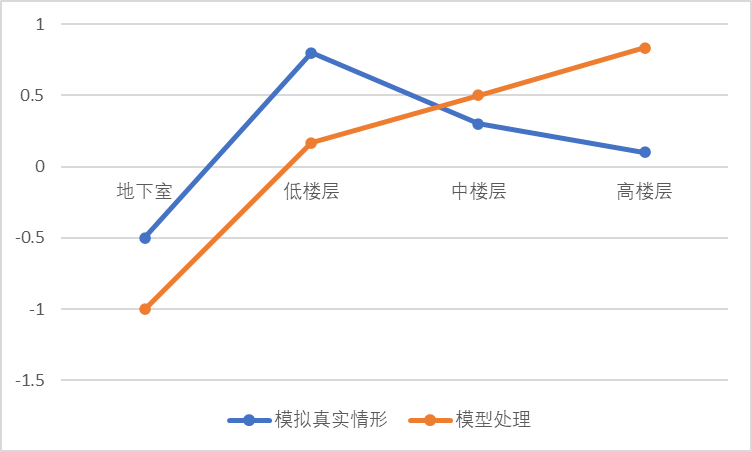
\includegraphics[width=0.7\textwidth]{figures/楼层.png}
    \caption{真实模拟的和模型处理的楼层分布对比}
    \label{fig:floor_distribution}
\end{figure}

由此可见两者之间的平行关系较差,拟合效果不好。

\textbf{(2) 梯户比例的处理}

\begin{lstlisting}[label=code:ratio_mapping, language=Python, caption=梯户比例的处理-中文数字到阿拉伯数字映射字典]
    # 1. 定义中文数字到阿拉伯数字的映射
    chinese_num_map = {
        '零': 0, '一': 1, '二': 2, '三': 3, '四': 4, '五': 5, '六': 6, '七': 7, '八': 8, '九': 9, '十': 10, '百': 100, '千': 1000, '万': 10000
    }
\end{lstlisting}

从代码\ref{code:ratio_mapping}中可以看到,遗漏了“两”到“2”的映射,会导致处理效果不好。

此外没有对梯户比例进行非线性的处理。由于梯户比例高于1之后,梯户比例的边际效用将会显著降低,所以应当对梯户比例大于1的部分进行弱化处理。
具体操作在后面建议部分已经提出。

\chapter{模型训练与预测}
在该部分,我们将对第2组同学建立的模型及其预测效果进行回归,以此来分析
OLS、Lasso、Ridge、ElasticNet模型在样本内外和交叉样本的表现效果。

\section{OLS模型}

\subsection{变量选取}
下面代码\ref{code:ols_features}中展示了第2组同学对数据进行特征选择的过程。

\begin{lstlisting}[label=code:ols_features, language=Python, caption=OLS模型特征选取]
    # 设置随机种子以确保结果的可复现性
    RANDOM_SEED = 42
    np.random.seed(RANDOM_SEED)
    random.seed(RANDOM_SEED)
    tf.random.set_seed(RANDOM_SEED)

    # 使用深度学习模型选择特征
    # 1. 深度学习特征选择 (使用MLP来选择重要特征)
    model = Sequential()
    model.add(Dense(256, input_dim=X_train_cleaned.shape[1], activation='relu'))
    model.add(Dense(128, activation='relu'))
    model.add(Dense(1, activation='linear'))

    # 编译和训练模型
    model.compile(optimizer='adam', loss='mean_squared_error', metrics=['mean_absolute_error'])
    model.fit(X_train_cleaned, y_train, epochs=20, batch_size=16, verbose=1)

    # 获取特征权重
    feature_weights = model.layers[0].get_weights()[0]
    feature_importance = np.mean(np.abs(feature_weights), axis=1)

    # 选择重要特征
    important_features = np.argsort(feature_importance)[-800:]
    X_train_selected = X_train_cleaned.iloc[:, important_features]
    X_test_selected = X_test_cleaned.iloc[:, important_features]

    # 2. 数据标准化
    scaler = StandardScaler()
    X_train_scaled = scaler.fit_transform(X_train_selected)
    X_test_scaled = scaler.transform(X_test_selected)
    # 3. PCA降维
    pca = PCA(n_components=0.999999, random_state=RANDOM_SEED)
    X_train_pca = pca.fit_transform(X_train_scaled)
    X_test_pca = pca.transform(X_test_scaled)
\end{lstlisting}

第2组的同学对于清洗后的数据,通过多层感知器(MLP)深度学习模型对特征重要性
进行评估,并根据特征的重要性,选择最重要的800个特征,从而得到两个新的数据集
\lstinline{X_train_selected}和\lstinline{X_test_selected},他们只包含这些重要的特征。
之后对这些特征数据进行标准化处理以为后续主成分分析法(PCA)做好准备,之后通过主成分分析法降维保留99.9999\%的方差,
目的是提高模型性能,减少过拟合,并提升训练效率(最终实现效果并不理想,在后续将逐渐进行介绍)。

经过第1组成员测定,第2组最终用于训练的变量个数为745,其实并未很好降维。
\subsection{模型训练与验证结果}

\begin{lstlisting}[label=code:ols_model, language=Python, caption=OLS模型训练]
    lr_best = LinearRegression()
    lr_best.fit(X_train_pca, y_train)

    train_lr_mae = mean_absolute_error(y_train, lr_best.predict(X_train_pca))   
    test_lr_mae = mean_absolute_error(y_test, lr_best.predict(X_test_pca))
    cv_lr_mae = -cross_val_score(lr_best, X_train_pca, y_train, cv=6, scoring='neg_mean_absolute_error').mean()
\end{lstlisting}

由此得出的OLS模型在样本内外以及交叉验证的MAE值如下表\ref{tab:ols_mae}所示:

\begin{table}[htbp]
    \centering
    \caption{OLS模型在样本内外以及交叉验证的MAE值}
    \label{tab:ols_mae}
    \scalebox{1.1}{
    \begin{tabular}{cccc}
        \toprule
        \multicolumn{1}{c}{ } & \multicolumn{1}{c}{样本内} & \multicolumn{1}{c}{交叉验证} & \multicolumn{1}{c}{样本外} \\
        \midrule
        MAE & 347313.52 & 352144.97 & 728837027.67 \\
        \bottomrule
    \end{tabular}
    }
\end{table}

训练集的MAE(347313.515636239)与测试集的MAE(352144.9672973303)相差不大,这表明模型在训练集和测试集上的表现相对一致。
这是一个好的迹象,因为它表明模型没有在训练集上过度拟合。
但6折交叉验证的MAE(728837027.6682167)远高于训练集和测试集的MAE。这表明模型在交叉验证集上的表现显著变差,这可能是过拟合的一个信号。

尽管训练集和测试集的MAE相近,但交叉验证的MAE异常高,这表明模型可能对训练数据过度拟合。这可能是因为模型在训练过程中学习到了训练数据中的噪声和细节,而没有很好地泛化到新的数据上。

原模型中,没有计算$R^2$和$Adj. R^2$,这里给出补充代码\ref{code:R^2}并计算:
\begin{lstlisting}[label=code:R^2, language=Python, caption=OLS模型样本内外和交叉验证的MAE、$R^2$、$Adj. R^2$计算]
    from sklearn.metrics import mean_absolute_error, r2_score
    from sklearn.model_selection import cross_val_predict, cross_val_score
    import numpy as np

    # 定义计算调整后R²的函数
    def adjusted_r2_score(y_true, y_pred, n, p):
        r2 = r2_score(y_true, y_pred)
        return 1 - (1 - r2) * (n - 1) / (n - p - 1)

    # 计算训练集和测试集上的MAE
    train_lr_mae = mean_absolute_error(y_train, lr_best.predict(X_train_pca))
    test_lr_mae = mean_absolute_error(y_test, lr_best.predict(X_test_pca))

    # 计算交叉验证集上的MAE
    cv_lr_mae = -cross_val_score(lr_best, X_train_pca, y_train, cv=6, scoring='neg_mean_absolute_error').mean()

    # 计算训练集上的R²和调整后R²
    train_lr_r2 = r2_score(y_train, lr_best.predict(X_train_pca))
    train_lr_adj_r2 = adjusted_r2_score(y_train, lr_best.predict(X_train_pca), len(y_train), X_train_pca.shape[1])

    # 计算测试集上的R²和调整后R²
    test_lr_r2 = r2_score(y_test, lr_best.predict(X_test_pca))
    test_lr_adj_r2 = adjusted_r2_score(y_test, lr_best.predict(X_test_pca), len(y_test), X_test_pca.shape[1])

    # 使用cross_val_predict获取交叉验证的预测结果
    y_pred_cv = cross_val_predict(lr_best, X_train_pca, y_train, cv=6)

    # 计算交叉验证集上的R²和调整后R²
    cv_lr_r2 = r2_score(y_train, y_pred_cv)
    cv_lr_adj_r2 = adjusted_r2_score(y_train, y_pred_cv, len(y_train), X_train_pca.shape[1])

    # 打印结果
    print(f"训练集 MAE: {train_lr_mae}")
    print(f"测试集 MAE: {test_lr_mae}")
    print(f"交叉验证 MAE: {cv_lr_mae}")
    print(f"训练集 R²: {train_lr_r2}")
    print(f"训练集 调整后 R²: {train_lr_adj_r2}")
    print(f"测试集 R²: {test_lr_r2}")
    print(f"测试集 调整后 R²: {test_lr_adj_r2}")
    print(f"交叉验证 R²: {cv_lr_r2}")
    print(f"交叉验证 调整后 R²: {cv_lr_adj_r2}")
\end{lstlisting}

结果展现如下表\ref{tab:ols_mae_r2}所示:

\begin{table}[htbp]
    \centering
    \caption{OLS模型在样本内外以及交叉验证的MAE、$R^2$、$Adj. R^2$}
    \label{tab:ols_mae_r2}
    \scalebox{1.1}{
    \begin{tabular}{cccc}
        \toprule
        \multicolumn{1}{c}{ } & \multicolumn{1}{c}{样本内} & \multicolumn{1}{c}{交叉验证} & \multicolumn{1}{c}{样本外} \\
        \midrule
        MAE & 347313.52 & 352144.97 & 728837027.67 \\
        $R^2$ & 0.7599 & 0.7686 & -13426487025.97 \\
        $Adj. R^2$ & 0.7577 & 0.7599 & -13550058410.15 \\
        \bottomrule
    \end{tabular}
    }
\end{table}

很明显在交叉验证过程中出现了异常数据的问题。

\section{Lasso}
\subsection{变量选取}
下面代码\ref{code:lasso_features}展示了第2组对Lasso模型的特征选择过程。
\begin{lstlisting}[label=code:lasso_features, language=Python, caption=Lasso模型特征选取]
    # 初始化Lasso模型,设置alpha参数  
    lasso = Lasso(alpha=10)  
    
    # 使用SelectFromModel进行特征选择  
    selector = SelectFromModel(lasso, threshold='median', prefit=False)  
    X_lasso_filtered = selector.fit_transform(X_train_cleaned, y_train)  
    
    print(f"原始特征数量: {X_train_cleaned.shape[1]}")  
    print(f"选择后的特征数量: {X_lasso_filtered.shape[1]}")
\end{lstlisting}

此处选用\lstinline{SelectFromModel}进行特征选择,核心思想是在模型既定的情况下学习出对提
高模型准确性最好的特征属性。具体而言,若某一Lasso模型特征的重要性(通过模型系
数的绝对值确定)低于其所用特征重要性的中间数,则舍弃这一特征;反之,则保留。
选取Lasso模型参数\lstinline{alpha=10},经变量筛选后,变量数量由原来的1018个下降为509个,
具体筛选结果如下表\ref{tab:lasso_features}所示:

重要性排名前10名的变量及其系数如图\ref{tab:lasso_features}所示:

\begin{table}[htbp]
    \centering
    \caption{Lasso特征重要性排名前10的变量及其系数}
    \label{tab:lasso_features}
    \scalebox{1.1}{%
    \begin{tabular}{ccc}
        \toprule
        \multicolumn{1}{c}{排名} & \multicolumn{1}{c}{变量名称} & \multicolumn{1}{c}{系数} \\
        \midrule
        1 & 板块\_406 & 2449770.03 \\
        2 & 区域\_18 & 2387008.96 \\
        3 & 板块\_475 & 1880121.66 \\
        4 & 板块\_30 & 1850492.92 \\
        5 & 板块\_486 & 1749190.27 \\
        6 & 板块\_515 & 1692133.68 \\
        7 & 板块\_530 & 1682903.94 \\
        8 & 房屋用途\_平房 & 1588970.08 \\
        9 & 板块\_279 & 1558026.61 \\
        10 & 区域\_52 & 1384402.90 \\
        \bottomrule
    \end{tabular}%
    }
\end{table}

特征选择过程中,保留数量最多的前5名特征前缀,结果如下表\ref{tab:feature_retention}所示。
(如特征变量为 板块\_515 ,则 板块 即为其“特征前缀”)

\begin{table}[htbp]
    \centering
    \caption{Lasso保留数量最多的前5名特征前缀}
    \label{tab:feature_retention}
    \scalebox{1.1}{% 将表格放大1.1倍
    \begin{tabular}{ccccc}
        \toprule
        \textbf{排名} & \textbf{特征前缀} & \textbf{保留数量} & \textbf{原有数量} & \textbf{保留比例} \\
        \midrule
        1 & 板块 & 368 & 453 & 81.24\% \\
        2 & 区域 & 62 & 74 & 83.78\% \\
        3 & 环线 & 12 & 13 & 92.31\% \\
        4 & 交易权属 & 8 & 9 & 88.89\% \\
        5 & 房屋用途 & 8 & 11 & 72.73\% \\
        \bottomrule
    \end{tabular}
    }
\end{table}

特征选择过程中,舍弃数量最多的前5名特征前缀,如下表\ref{tab:feature_discarding}所示:
\begin{table}[htbp]
    \centering
    \caption{Lasso舍弃数量最多的前5名特征前缀}
    \label{tab:feature_discarding}
    \scalebox{1.1}{% 将表格放大1.1倍
    \begin{tabular}{ccccc}
        \toprule
        \textbf{排名} & \textbf{特征前缀} & \textbf{舍弃数量} & \textbf{原有数量} & \textbf{舍弃比例} \\
        \midrule
        1 & 核心卖点 & 100 & 100 & 100.00\% \\
        2 & 周边配套 & 96 & 100 & 96.00\% \\
        3 & 交通出行 & 96 & 100 & 96.00\% \\
        4 & 户型介绍 & 94 & 100 & 94.00\% \\
        5 & 板块 & 85 & 453 & 18.76\% \\
        \bottomrule
    \end{tabular}
    }
\end{table}

代码(\ref{code:lasso_features_evaluation}、\ref{code:lasso_features_discarding})
从第2组的模型中获取了上方表
(\ref{tab:lasso_features}、\ref{tab:feature_retention}、\ref{tab:feature_discarding})中所示的内容。
\begin{lstlisting}[label=code:lasso_features_evaluation, language=Python, caption=Lasso:重要性排名前10的变量及其系数]
    coefficients = lasso_best.coef_
    selected_features_bool = selector.get_support()
    feature_names = X_train_cleaned.columns.tolist()

    selected_feature_names = [feature_names[i] for i in range(len(feature_names)) if selected_features_bool[i]]

    # 按系数绝对值大小排序
    sorted_features = sorted(zip(coefficients, selected_feature_names), key=lambda x: abs(x[0]), reverse=True)

    print("前10个重要性最高的变量及其系数:")
    for coef, name in sorted_features[:10]:
        print(f"{name}: {coef}")
\end{lstlisting}

\begin{lstlisting}[label=code:lasso_features_discarding, language=Python, caption=Lasso:查看特征选择过程中保留与舍弃的特征]
    from collections import Counter
    import heapq
    
    feature_names = X_train_cleaned.columns.tolist()
    
    selected_features = selector.get_support(indices=True)
    
    all_feature_names = feature_names
    
    # 获取保留的特征名称和舍弃的特征名称
    selected_feature_names = [all_feature_names[i] for i in selected_features]
    dropped_feature_names = [all_feature_names[i] for i in range(X_train_cleaned.shape[1]) if i not in selected_features]
    
    # 统计所有特征前缀、保留的特征前缀和舍弃的特征前缀
    all_prefixes = Counter([feature.split('_')[0] for feature in all_feature_names])
    selected_prefixes = Counter([feature.split('_')[0] for feature in selected_feature_names])
    dropped_prefixes = Counter([feature.split('_')[0] for feature in dropped_feature_names])
    
    # 获取前5个保留最多的特征前缀及其数量和比例
    most_selected_prefixes = heapq.nlargest(5, selected_prefixes.items(), key=lambda x: x[1])
    
    # 获取前5个舍弃最多的特征前缀及其数量和比例
    most_dropped_prefixes = heapq.nlargest(5, dropped_prefixes.items(), key=lambda x: x[1])
    
    # 输出前5个保留最多的特征前缀及其数量、原有数量和比例的表格
    print("\n前5个保留最多的特征前缀、保留数量、原有数量及其占其原有数量的比例:")
    print(f"{'特征前缀':<20}{'保留数量':>10}{'原有数量':>10}{'保留比例':>10}")
    for prefix, selected_count in most_selected_prefixes:
        total_count = all_prefixes[prefix]
        ratio = selected_count / total_count
        print(f"{prefix:<20}{selected_count:>10}{total_count:>10}{ratio:>10.2%}")
    
    # 输出前5个舍弃最多的特征前缀、丢弃数量、原有数量及其占其原有数量的比例的表格
    print("\n前5个舍弃最多的特征前缀、丢弃数量、原有数量及其占其原有数量的比例:")
    print(f"{'特征前缀':<20}{'舍弃数量':>10}{'原有数量':>10}{'舍弃比例':>10}")
    for prefix, dropped_count in most_dropped_prefixes:
        total_count = all_prefixes[prefix]
        ratio = dropped_count / total_count
        print(f"{prefix:<20}{dropped_count:>10}{total_count:>10}{ratio:>10.2%}")
\end{lstlisting}

可以看到,对lasso模型较为重要的特征多为板块、区域类特征,而核心卖点、周边配套、交通出行与户型介绍则为舍弃较多的特征,
表明它们对模型的预测贡献不大,特别是“核心卖点”特征的舍弃比例已高达100\%,
可能是由于当前数据处理方法并未准确捕捉数据蕴含的有用信息,需要更细致的预处理,
如去除停用词、词干提取(Stemming)或词形还原(Lemmatization),以减少噪声并提高特征的质量,
可考虑通过不同的特征工程方法来更好地捕捉这些特征的信息,例如使用词袋模型(Bag of Words)、
TF-IDF或基于深度学习的BERT嵌入等其他文本分析方法,也可考虑递归特征消除(RFE)等其他特征选择方法。

\subsection{模型训练与验证结果}
下面代码\ref{code:lasso_model}展示了第2组Lasso模型训练及验证的代码:
\begin{lstlisting}[label=code:lasso_model, language=Python, caption=Lasso模型训练]
    #训练模型
    lasso_best = Lasso(alpha=10)
    lasso_best.fit(X_lasso_filtered,y_train)
    # 在训练集上进行预测  
    train_predictions = lasso_best.predict(X_lasso_filtered)  
    # 计算训练集的MAE
    train_lasso_mae = mean_absolute_error(y_train, train_predictions)  
    print(f"Training MAE: {train_lasso_mae}")  
    # 计算训练集的R²  
    train_lasso_r2 = r2_score(y_train, train_predictions)  
    print(f"Training R²: {train_lasso_r2}")

    # 交叉验证
    cv_predictions = cross_val_predict(lasso_best,X_lasso_filtered, y_train, cv=6)  

    cv_lasso_mae = mean_absolute_error(y_train, cv_predictions)  
    print(f"Cross-validated MAE: {cv_lasso_mae}")   
    cv_lasso_r2 = r2_score(y_train, cv_predictions)  
    print(f"Cross-validated R²: {cv_lasso_r2}")
\end{lstlisting}

结合上下文分析,代码中可能存在一处错误:最后的\lstinline|print(f"Training R²: {test_lasso_r2}")|应为\lstinline|print(f"Test R²: {test_lasso_r2}")|。

选取参数\lstinline{alpha=10}进行模型训练与与预测,lasso模型在样本内、样本外及交叉验证时的表现如下表\ref{tab:lasso_mae_r2}所示:
\begin{table}[htbp]
    \centering
    \caption{Lasso模型在样本内、样本外及交叉验证时的表现}
    \label{tab:lasso_mae_r2}
    \scalebox{1.1}{
    \begin{tabular}{cccc}
        \toprule
        \multicolumn{1}{c}{ } & \multicolumn{1}{c}{样本内} & \multicolumn{1}{c}{交叉验证} & \multicolumn{1}{c}{样本外} \\
        \midrule
        MAE & 346088.67 & 350422.06 & 348936.58 \\
        $R^2$ & 0.7581 & 0.7677 & 0.7526 \\
        $Adj. R^2$ & 0.7566 & 0.7618 & 0.7566 \\
        \bottomrule
    \end{tabular}
    }
\end{table}

数据显示,Lasso模型的MAE约为35万元,拟合优度约为75\%,整体而言模型表现较好。

为更直观的展现模型,我们绘制了lasso模型在训练集上的残差图,如下图\ref{fig:lasso_residual}、\ref{fig:lasso_residual_interval}所示:

\begin{figure}[H]
    \centering
    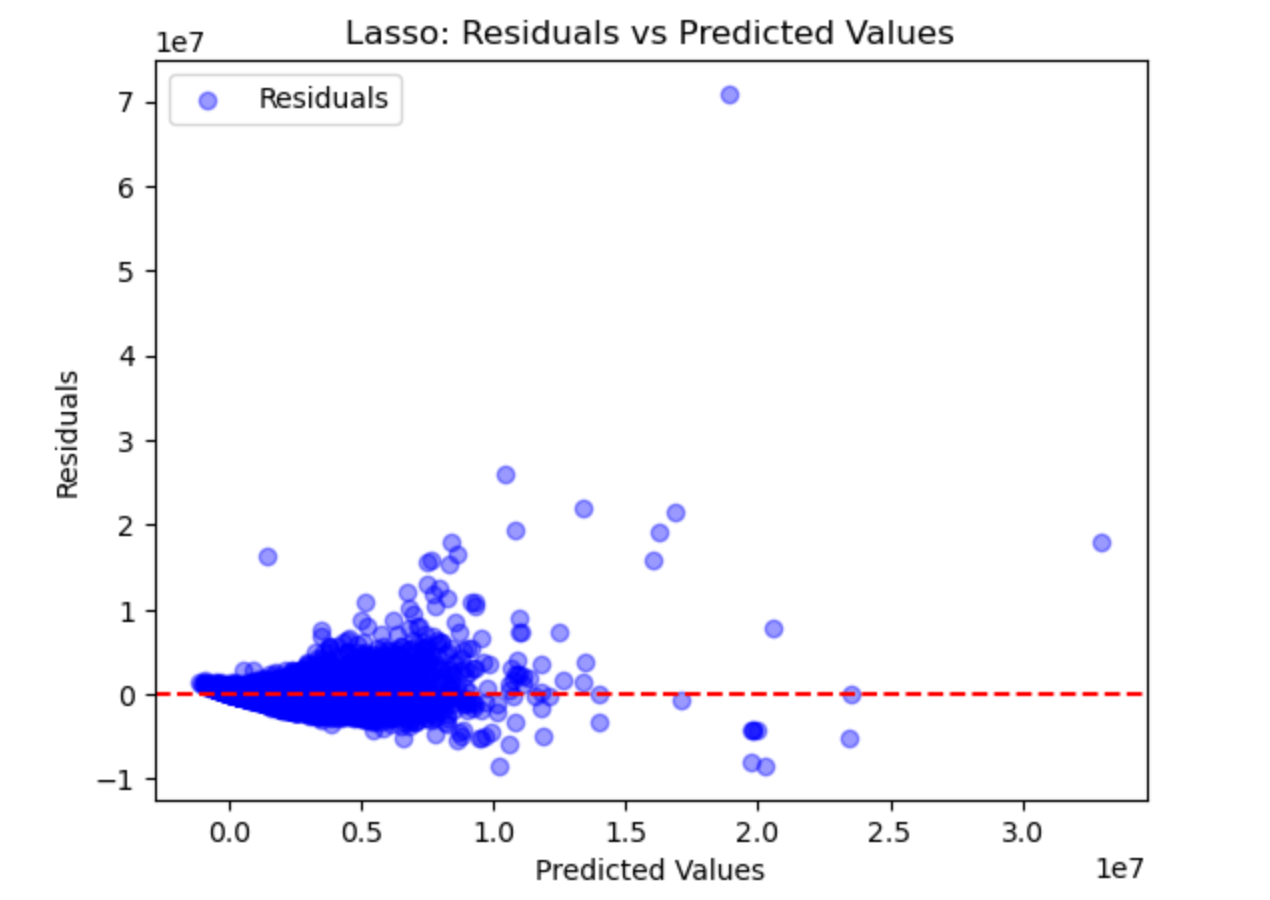
\includegraphics[width=0.8\textwidth]{figures/lasso-残差图.png}
    \caption{Lasso模型在训练集上的残差图}
    \label{fig:lasso_residual}
\end{figure}

\begin{figure}[H]
    \centering
    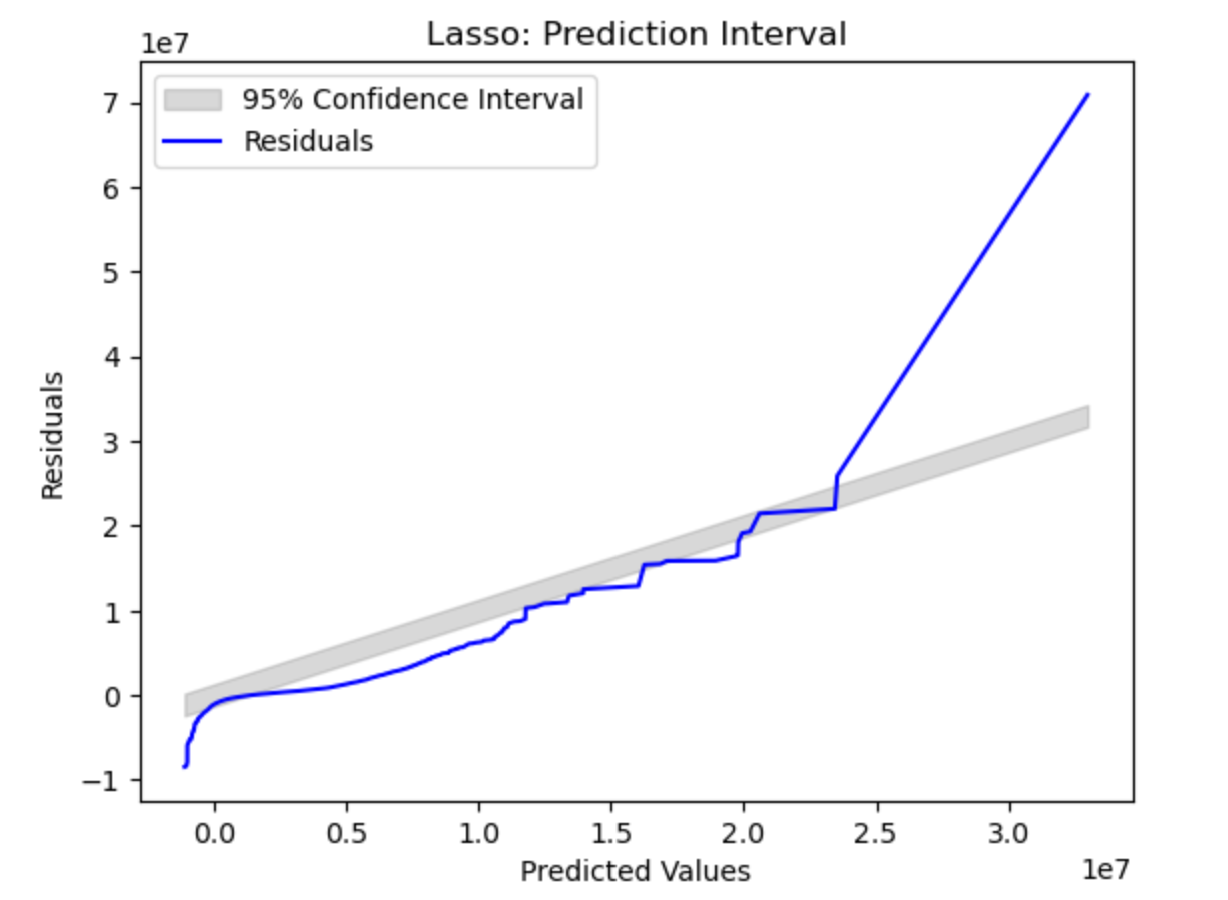
\includegraphics[width=0.8\textwidth]{figures/lasso-置信区间.png}
    \caption{Lasso模型在训练集上的残差与95\%置信区间}
    \label{fig:lasso_residual_interval}
\end{figure}

残差图显示,多数残差集中在预测值的较低区间(0到1.5*1e7)并围绕零线随机分布,
表明模型在这一范围内的预测相对准确;但残差的分布并不均匀,而是随着预测值的增大
而增加,表明可能存在异方差性。此外,图中有离群点,表明数据中可能存在异常值,
对模型的拟合质量构成影响。整体而言,模型在较低预测值范围内的拟合效果较好,
但在处理较高预测值时可能需要进一步优化。
\newpage

\begin{lstlisting}[label=code:lasso_residual, language=Python, caption=Lasso模型残差可视化图\ref{fig:lasso_residual}补充代码]
    import matplotlib.pyplot as plt
    import numpy as np
    from scipy.stats import linregress

    # 绘制残差图
    plt.scatter(train_predictions, y_train - train_predictions, color='blue',alpha=0.4, label='Residuals')
    # 添加零线
    plt.axhline(y=0, color='r', linestyle='--', linewidth=1.5)

    plt.xlabel('Predicted Values')
    plt.ylabel('Residuals')
    plt.title('Residuals vs Predicted Values')
    plt.legend(loc='upper left')
    plt.show()
\end{lstlisting}

\begin{lstlisting}[label=code:lasso_residual_interval, language=Python, caption=Lasso模型残差与95\%置信区间可视化图\ref{fig:lasso_residual_interval}补充代码]
    import matplotlib.pyplot as plt
    import numpy as np
    from sklearn.metrics import mean_squared_error
    
    # 模型的预测区间
    std_err = np.sqrt(mean_squared_error(y_train, train_predictions))
    conf_int = 1.96 * std_err
    plt.fill_between(np.sort(train_predictions), 
                     np.sort(train_predictions) - conf_int, np.sort(train_predictions) + conf_int, color='gray', 
                     alpha=0.3, label='95% Confidence Interval')
    plt.plot(np.sort(train_predictions), np.sort(y_train - train_predictions), color='blue', label='Residuals')
    plt.xlabel('Predicted Values')
    plt.ylabel('Residuals')
    plt.title('Prediction Interval')
    plt.legend(loc='best')
    plt.show()
\end{lstlisting}

\section{Ridge}
\subsection{变量选取}
下面代码\ref{code:ridge_features}展示了第3组Ridge模型的特征选择过程。
\begin{lstlisting}[label=code:ridge_features, language=Python, caption=Ridge模型特征选取]
    # 初始化Lasso模型,设置alpha参数  
    ridge = Ridge(alpha=10)  
      
    # 使用SelectFromModel进行特征选择  
    selector_ridge = SelectFromModel(ridge, threshold='median', prefit=False)  
    X_ridge_filtered = selector_ridge.fit_transform(X_train_cleaned, y_train)  
      
    print(f"原始特征数量: {X_train_cleaned.shape[1]}")  
    print(f"选择后的特征数量: {X_ridge_filtered.shape[1]}")
\end{lstlisting}

根据上下文分析,第一行的代码注释中可能有一处错误:“初始化Lasso模型”应为“初始化Ridge模型”。

此处沿用\lstinline{SelectFromModel}这一特征选择方法,基于ridge模型选择出对提高模型准确性最好的特征。
选取模型参数\lstinline{alpha=10},经变量筛选后,变量数量由原来的1018个下降为509个,具体筛选情况如下:

Ridge模型的特征重要性排名前10的变量及其系数如下表\ref{tab:variables_coefficients}所示:

\begin{table}[htbp]
    \centering
    \caption{Ridge特征重要性排名前10的变量及其系数}
    \label{tab:variables_coefficients}
    \scalebox{1.1}{%
    \begin{tabular}{ccc}
        \toprule
        \textbf{排名} & \textbf{变量名称} & \textbf{系数} \\
        \midrule
        1 & 区域\_18 & 2143269.88 \\
        2 & 板块\_530 & 1573203.59 \\
        3 & 区域\_52 & 1413229.61 \\
        4 & 板块\_486 & 1340104.11 \\
        5 & 板块\_30 & 1328557.30 \\
        6 & 板块\_279 & 1264602.27 \\
        7 & 板块\_11 & 1113019.43 \\
        8 & 板块\_9 & -1086304.54 \\
        9 & 板块\_504 & 1049970.23 \\
        10 & 板块\_269 & 1014432.41 \\
        \bottomrule
    \end{tabular}%
    }
\end{table}

特征选择过程中,保留数量最多的前5名特征前缀如下表\ref{tab:feature_retention_ridge}所示:
\begin{table}[htbp]
    \centering
    \caption{Ridge特征保留情况}
    \label{tab:feature_retention_ridge}
    \begin{tabular}{ccccc}
        \toprule
        \textbf{排名} & \textbf{特征前缀} & \textbf{保留数量} & \textbf{原有数量} & \textbf{保留比例} \\
        \midrule
        1 & 板块 & 368 & 453 & 81.24\% \\
        2 & 区域 & 62 & 74 & 83.78\% \\
        3 & 环线 & 12 & 13 & 92.31\% \\
        4 & 交易权属 & 8 & 9 & 88.89\% \\
        5 & 房屋用途 & 8 & 11 & 72.73\% \\
        \bottomrule
    \end{tabular}
\end{table}

特征选择过程中,保留数量最多的前5名特征前缀如下表\ref{tab:feature_discarding_ridge}所示:

\begin{table}[htbp]
    \centering
    \caption{Ridge特征舍弃情况}
    \label{tab:feature_discarding_ridge}
    \begin{tabular}{ccccc}
        \toprule
        \textbf{排名} & \textbf{特征前缀} & \textbf{舍弃数量} & \textbf{原有数量} & \textbf{舍弃比例} \\
        \midrule
        1 & 核心卖点 & 100 & 100 & 100.00\% \\
        2 & 周边配套 & 96 & 100 & 96.00\% \\
        3 & 交通出行 & 96 & 100 & 96.00\% \\
        4 & 户型介绍 & 94 & 100 & 94.00\% \\
        5 & 板块 & 85 & 453 & 18.76\% \\
        \bottomrule
    \end{tabular}
\end{table}

上方表(\ref{tab:variables_coefficients}、\ref{tab:feature_retention_ridge}、\ref{tab:feature_discarding_ridge})用到的提取代码如下
代码(\ref{code:feature_selection_ridge}、\ref{code:feature_retention_ridge})所示:
\begin{lstlisting}[label=code:feature_selection_ridge, language=Python, caption=Ridge:重要性排名前10的变量及其系数]
    coefficients = ridge_best.coef_
    selected_features_bool = selector_ridge.get_support()
    feature_names = X_train_cleaned.columns.tolist()
    selected_feature_names = [feature_names[i] for i in range(len(feature_names)) if selected_features_bool[i]]
    # 按系数绝对值大小排序
    sorted_features = sorted(zip(coefficients, selected_feature_names), key=lambda x: abs(x[0]), reverse=True)
    
    print("前10个重要性最高的变量及其系数:")
    for coef, name in sorted_features[:10]:
        print(f"{name}: {coef}")
\end{lstlisting}

\begin{lstlisting}[label=code:feature_retention_ridge, language=Python, caption=Ridge:Ridge:查看特征选择过程中保留与舍弃的特征]
    from collections import Counter
    import heapq
    
    feature_names = X_train_cleaned.columns.tolist()
    ridge_selected_features = selector_ridge.get_support(indices=True)
    all_feature_names = feature_names
    
    # 获取保留的特征名称和舍弃的特征名称
    ridge_selected_feature_names = [all_feature_names[i] for i in selected_features]
    ridge_dropped_feature_names = [all_feature_names[i] for i in range(X_train_cleaned.shape[1]) if i not in selected_features]
    
    # 统计所有特征前缀、保留的特征前缀和舍弃的特征前缀
    ridge_all_prefixes = Counter([feature.split('_')[0] for feature in all_feature_names])
    ridge_selected_prefixes = Counter([feature.split('_')[0] for feature in ridge_selected_feature_names])
    ridge_dropped_prefixes = Counter([feature.split('_')[0] for feature in ridge_dropped_feature_names])
    
    # 获取前5个保留最多的特征前缀及其数量和比例
    ridge_most_selected_prefixes = heapq.nlargest(5, ridge_selected_prefixes.items(), key=lambda x: x[1])
    
    # 获取前5个舍弃最多的特征前缀及其数量和比例
    ridge_most_dropped_prefixes = heapq.nlargest(5, ridge_dropped_prefixes.items(), key=lambda x: x[1])
    
    # 输出前5个保留最多的特征前缀及其数量、原有数量和比例的表格
    print("\n前5个保留最多的特征前缀、保留数量、原有数量及其占其原有数量的比例:")
    print(f"{'特征前缀':<20}{'保留数量':>10}{'原有数量':>10}{'保留比例':>10}")
    for prefix, selected_count in ridge_most_selected_prefixes:
        total_count = all_prefixes[prefix]
        ratio = selected_count / total_count
        print(f"{prefix:<20}{selected_count:>10}{total_count:>10}{ratio:>10.2%}")
    
    # 输出前5个舍弃最多的特征前缀、丢弃数量、原有数量及其占其原有数量的比例的表格
    print("\n前5个舍弃最多的特征前缀、丢弃数量、原有数量及其占其原有数量的比例:")
    print(f"{'特征前缀':<20}{'舍弃数量':>10}{'原有数量':>10}{'舍弃比例':>10}")
    for prefix, dropped_count in ridge_most_dropped_prefixes:
        total_count = all_prefixes[prefix]
        ratio = dropped_count / total_count
        print(f"{prefix:<20}{dropped_count:>10}{total_count:>10}{ratio:>10.2%}")
\end{lstlisting}

可以看到,和Lasso模型的情况类似,对Ridge模型较为重要的特征多为板块、区域类特征,
而核心卖点、周边配套、交通出行与户型介绍则为舍弃较多的特征,“核心卖点”特征的舍弃比例仍为100\%,
与Lasso模型结果的结论所反映的问题一致,文本数据可能需要更为细致的预处理过程。

\subsection{模型训练与验证结果}
\begin{lstlisting}[label=code:ridge_model, language=Python, caption=Ridge模型训练]
    ridge_best = Ridge(alpha=10)  # 可以调整alpha值  
    ridge_best.fit(X_ridge_filtered, y_train)  

    # 在训练集上进行预测  
    train_predictions = ridge_best.predict(X_ridge_filtered) 
    # 计算MAE
    train_ridge_mae = mean_absolute_error(y_train, train_predictions)  
    print(f"Training MAE: {train_ridge_mae}")  
    # 计算训练集的R²  
    train_ridge_r2 = r2_score(y_train, train_predictions)  
    print(f"Training R²: {train_ridge_r2}")

    # 交叉验证
    cv_predictions = cross_val_predict(ridge_best,X_ridge_filtered, y_train, cv=6)  

    cv_ridge_mae = mean_absolute_error(y_train, cv_predictions)  
    print(f"Cross-validated MAE: {cv_ridge_mae}")   
    cv_ridge_r2 = r2_score(y_train, cv_predictions)  
    print(f"Cross-validated R²: {cv_ridge_r2}")

    # 在测试集上进行预测
    X_test_filtered = selector_ridge.transform(X_test_cleaned) 
    test_predictions = ridge_best.predict(X_test_filtered)  

    test_ridge_mae = mean_absolute_error(y_test, test_predictions)  
    print(f"Test MAE: {test_ridge_mae}") 
    test_ridge_r2 = r2_score(y_test, test_predictions)  
    print(f"Training R²: {train_ridge_r2}")
\end{lstlisting}

结合代码上下文分析,代码中可能存在一处错误:
最后的\lstinline|print(f"Training R²: {test_lasso_r2}")|应为\lstinline|print(f"Test R²: {test_lasso_r2}")|。

选取模型参数\lstinline|alpha=10|进行模型训练与预测,Ridge模型在样本内、样本外及交叉验证时的表现如下表\ref{tab:ridge_mae_r2}所示:
\begin{table}[htbp]
    \centering
    \caption{Ridge模型在样本内、样本外及交叉验证时的表现}
    \label{tab:ridge_mae_r2}
    \scalebox{1.1}{
    \begin{tabular}{cccc}
        \toprule
        \multicolumn{1}{c}{ } & \multicolumn{1}{c}{样本内} & \multicolumn{1}{c}{交叉验证} & \multicolumn{1}{c}{样本外} \\
        \midrule
        MAE & 346778.86 & 350795.78 & 349140.23 \\
        $R^2$ & 0.7557 & 0.7557 & 0.7511 \\
        $Adj. R^2$ & 0.7542 & 0.7598 & 0.7542 \\
        \bottomrule
    \end{tabular}
    }
\end{table}

数据表明,Ridge模型的MAE约为35万元,拟合优度约为75\%,
与Lasso模型表现相当;模型在样本内、样本外及交叉验证时的表现接近,表明模型有较好的泛化能力,未出现过拟合现象。

为更直观的展现模型,我们绘制了Ridge模型在训练集上的残差图,如下图\ref{fig:Ridge_residual}、\ref{fig:Ridge_residual_interval}所示:

\begin{figure}[H]
    \centering
    \includegraphics[width=0.8\textwidth]{figures/Ridge-残差图.png}
    \caption{Ridge模型在训练集上的残差图}
    \label{fig:Ridge_residual}
\end{figure}

\begin{figure}[H]
    \centering
    \includegraphics[width=0.8\textwidth]{figures/Ridge-置信区间.png}
    \caption{Ridge模型在训练集上的残差与95\%置信区间}
    \label{fig:Ridge_residual_interval}
\end{figure}

残差图结果与Lasso模型的结果类似,这表明Ridge模型在较低预测值范围内的拟合效果较好,
但可能存在异常值与异方差性的问题,需要进一步优化。

作图代码如下代码(\ref{code:ridge_residual}、\ref{code:ridge_residual_interval})所示:
\begin{lstlisting}[label=code:ridge_residual, language=Python, caption=Ridge模型训练集残差可视化图\ref{fig:Ridge_residual}]
    # 绘制残差图
    plt.scatter(train_predictions, y_train - train_predictions, color='blue',alpha=0.4, label='Residuals')
    plt.axhline(y=0, color='r', linestyle='--', linewidth=1.5)
    
    plt.xlabel('Predicted Values')
    plt.ylabel('Residuals')
    plt.title('Ridge: Residuals vs Predicted Values')
    plt.legend(loc='upper left')
    plt.show()
\end{lstlisting}
\begin{lstlisting}[label=code:ridge_residual_interval, language=Python, caption=Ridge模型训练集残差与95\%置信区间可视化图\ref{fig:Ridge_residual_interval}]
    std_err = np.sqrt(mean_squared_error(y_train, train_predictions))
    conf_int = 1.96 * std_err
    plt.fill_between(np.sort(train_predictions), 
                     np.sort(train_predictions) - conf_int, np.sort(train_predictions) + conf_int, color='gray', 
                     alpha=0.3, label='95% Confidence Interval')
    plt.plot(np.sort(train_predictions), np.sort(y_train - train_predictions), color='blue', label='Residuals')
    plt.xlabel('Predicted Values')
    plt.ylabel('Residuals')
    plt.title('Ridge: Prediction Interval')
    plt.legend(loc='best')
    plt.show()
\end{lstlisting}

\section{ElasticNet}

\subsection{变量选取}
第2组ElasticNet所用的训练和测试数据依旧为pca降维后的745个变量,
选取\lstinline|alpha=0.001|及\lstinline|l1_ratio=0.5|进行训练。

\subsection{模型训练与验证结果}

\begin{lstlisting}[label=code:elasticnet_model, language=Python, caption=ElasticNet模型训练]
    en = ElasticNet(alpha=0.001, l1_ratio=0.5, max_iter=3000, random_state=42)
    en.fit(X_train_pca, y_train)
    train_en_mae = mean_absolute_error(y_train, en.predict(X_train_pca))   
    test_en_mae = mean_absolute_error(y_test, en.predict(X_test_pca))
    cv_en_mae = -cross_val_score(en, X_train_pca, y_train, cv=6, scoring='neg_mean_absolute_error').mean()
\end{lstlisting}

训练结果因为没有做出完整的指标显示,代码经过第1组补充后展示如下:
\begin{lstlisting}[label=code:elasticnet_R^2, language=Python, caption=ElasticNet模型样本内外和交叉验证的MAE、$R^2$、$Adj. R^2$计算]
    from sklearn.metrics import mean_absolute_error, r2_score
    from sklearn.model_selection import cross_val_predict, cross_val_score
    
    # 使用上述已经定义的计算调整后R²的函数,此处不再重复定义
    
    # 计算训练集和测试集上的MAE
    train_en_mae = mean_absolute_error(y_train, en.predict(X_train_pca))
    test_en_mae = mean_absolute_error(y_test, en.predict(X_test_pca))
    
    # 计算交叉验证集上的MAE
    cv_en_mae = -cross_val_score(en, X_train_pca, y_train, cv=6, scoring='neg_mean_absolute_error').mean()
    
    # 计算训练集上的R²和调整后R²
    train_en_r2 = r2_score(y_train, en.predict(X_train_pca))
    train_en_adj_r2 = adjusted_r2_score(y_train, en.predict(X_train_pca), len(y_train), X_train_pca.shape[1])
    
    # 计算测试集上的R²和调整后R²
    test_en_r2 = r2_score(y_test, en.predict(X_test_pca))
    test_en_adj_r2 = adjusted_r2_score(y_test, en.predict(X_test_pca), len(y_test), X_test_pca.shape[1])
    
    # 使用cross_val_predict获取交叉验证的预测结果
    y_pred_cv = cross_val_predict(en, X_train_pca, y_train, cv=6)
    
    # 计算交叉验证集上的R²和调整后R²
    cv_en_r2 = r2_score(y_train, y_pred_cv)
    cv_en_adj_r2 = adjusted_r2_score(y_train, y_pred_cv, len(y_train), X_train_pca.shape[1])
    
    # 打印结果
    print(f"训练集 MAE: {train_en_mae}")
    print(f"测试集 MAE: {test_en_mae}")
    print(f"交叉验证 MAE: {cv_en_mae}")
    print(f"训练集 R²: {train_en_r2}")
    print(f"训练集 调整后 R²: {train_en_adj_r2}")
    print(f"测试集 R²: {test_en_r2}")
    print(f"测试集 调整后 R²: {test_en_adj_r2}")
    print(f"交叉验证 R²: {cv_en_r2}")
    print(f"交叉验证 调整后 R²: {cv_en_adj_r2}")
\end{lstlisting}

因第2组该模型运行特别缓慢,最后只得到了一部分结果,如下展示:

\begin{table}[htbp]
    \centering
    \caption{ElasticNet模型在样本内、样本外及交叉验证时的MAE表现}
    \label{tab:elasticnet_mae_r2}
    \scalebox{1.1}{
    \begin{tabular}{cccc}
        \toprule
        \multicolumn{1}{c}{ } & \multicolumn{1}{c}{样本内} & \multicolumn{1}{c}{交叉验证} & \multicolumn{1}{c}{样本外} \\
        \midrule
        MAE & 347143.95 & 351833.19 & 351547.85 \\
        \bottomrule
    \end{tabular}
    }
\end{table}

训练集的MAE(347143.95)与测试集的MAE(351833.19)非常接近。这表明模型在训练集和测试集上的表现相对一致,
没有明显的过拟合现象。同时,交叉验证的MAE(351547.85)与训练集和测试集的MAE相差不大。这进一步表明模型具有较好的泛化能力。

\chapter{项目优化建议}

\section{数据处理部分}

\subsection{房屋户型的处理}

此模型使用中位数填补“室”“厅”缺失值,使用1填补“厨”“卫”缺失值。此方法不失为一种简便高效的处理方法。然而在此需要指出,存在一种更为有效的方式:通过回归特定房间数量与建筑面积之间的关系:
\begin{align}
    \text{Linear Regression:}\quad\text{Number of Room}=\alpha+\beta\times area
\end{align}

下面代码\ref{code:room_regression}给出了针对这一想法的实现代码:

\begin{lstlisting}[label=code:room_regression, language=Python, caption=房屋户型的处理修改代码]
    df['建筑面积'] = df['建筑面积'].str.replace('㎡', '').astype(float)
    train_huxing = df[(df[['房屋数量', '客厅数量', '厨房数量', '卫生间数量']] != 0).all(axis=1)]
    X_train = train_huxing[['建筑面积']]  # 输入特征是建筑面积
    Y_train_house = train_huxing['房屋数量']  # 输出标签是房屋数量
    Y_train_living = train_huxing['客厅数量']  # 输出标签是客厅数量
    Y_train_kitchen = train_huxing['厨房数量']  # 输出标签是厨房数量
    Y_train_bath = train_huxing['卫生间数量']  # 输出标签是卫生间的数量
    model_house = LinearRegression()
    model_living = LinearRegression()
    model_kitchen = LinearRegression()
    model_bath = LinearRegression()
    model_house.fit(X_train, Y_train_house)
    model_living.fit(X_train, Y_train_living)
    model_kitchen.fit(X_train, Y_train_kitchen)
    model_bath.fit(X_train, Y_train_bath)
    missing_data = df[(df[['房屋数量', '客厅数量', '厨房数量', '卫生间数量']] == 0).any(axis=1)    ]
    X_missing = missing_data[['建筑面积']]
    df.loc[X_missing.index, '房屋数量'] = np.round(model_house.predict(X_missing)).astype(int)
    df.loc[X_missing.index, '客厅数量'] = np.round(model_living.predict(X_missing)).astype(int)
    df.loc[X_missing.index, '厨房数量'] = np.round(model_kitchen.predict(X_missing)).astype(int)
    df.loc[X_missing.index, '卫生间数量'] = np.round(model_bath.predict(X_missing)).astype(int)
\end{lstlisting}

\subsection{梯户比例的优化}

最好对处理好的梯户比例数据进行非线性的处理:这是由于梯户比例高于1之后,梯户比例的边际效用将会显著降低。可以考虑构建一个函数来弱化大于1的部分的贡献,例如:
\begin{align}
    \text{disposed ratio}=\begin{cases}\text{original ratio},\quad\text{original ratio}\leq1\\
        2-\frac{1}{\text{original ratio}} ,\quad\text{original ratio}>1\end{cases}
\end{align}

这个映射将$[0,\infty)$映射到了$[0,2]$,相比原数据解释力更强一些。

同时,在过程中我们会遇到“五梯二十二户、七梯十四户”等这样的特殊情况,可以选择采用\lstinline|cn2an|库进行转化,
转化效率较高且准确度相对较高。

\subsection{所在楼层的处理}

我们团队认为最佳的处理方法是按低、中、高、地下室分离出4个示性变量,单独考虑每一项的效应。如果考虑变量降维,意图减少变量数量,可以对楼层保留线性处理,但是地下室必须单独提取为示性变量。

\subsection{布尔特征的适当运用}

将文本特征转换为布尔特征可能会丢失一些信息,例如文本中的数量或强度等。而且单纯的布尔特征可能无法表达特征间的组合关系,例如“东南”和“东”同时出现可能表示一个特定的区域,但单独的布尔特征无法表达这种组合关系。如果特征很多,转换后的布尔特征空间还可能会非常大,导致维度灾难,增加模型训练的难度和计算成本。

建议考虑引入权重系统,例如在房屋朝向的处理上,将方向的强度和权重数值化,例如给复合方向的权重设置为中间值0.4。


\subsection{缺失值填充方法的选择优化}

以房屋年限的处理为例。房屋年限的数据是随机的,中位数填充可能会影响数据的分布,引起偏差。且将“满两年”映射为2,“满五年”映射为5,可能会让人误以为这些数值代表具体的年数,且这样的映射主观认为房价和房屋年限存在线性关系,可能导致模型的误差。

建议使用哑变量,并保留原始分类特征。

下面代码\ref{code:room_regression}给出了以房屋年限为例的缺失值补充办法:

\begin{lstlisting}[label=code:room_regression, language=Python, caption=房屋年限处理改进建议]
    # 构造dummy variable
    df['满两年'] = 0
    df['满五年'] = 0
    def set_due_time(row):
        if row['房屋年限'] == '满五年':
            row['满五年'] = 1
        elif row['房屋年限'] == '满两年':
            row['满两年'] = 1
        return row
    df = df.apply(set_due_time, axis=1)
    df.drop('房屋年限', axis=1, inplace=True)
\end{lstlisting}

\subsection{details数据缺失}

建议使用details中的数据,第2组在进行数据处理的过程中完全没有应用到details数据,
这会导致模型丧失了一部分方差解释能力。

details中的数据包含小区规模、物业费、水电费、供暖类型、燃气费、供暖费等重要的指标,
这些指标一方面可以加入到模型中去,来更好解释房价;另一方面依据小区,可以补充一部分train中的缺失数据;意义重大。

因为此处只需要\lstinline|merge|操作,此处不再提供详细代码。

\section{模型训练与预测部分}

\subsection{特征选择}

第2组对于OLS、ElasticNet与Lasso、Ridge模型采用了不同的特征筛选方法,前者基于多层感知器深度学习模型选择了800个特征,
后者基于SelectFromModel方法选择了509个特征,考虑到不同的特征选择策略可能造成模型表现间的不可比,建议通过交叉验证等方法来评估各特征选择策略的效果,选择一个最佳方案。我们也给出一些其他的特征选择策略可供考量:

\begin{itemize}
    \item \textbf{递归特征消除(RFE):}递归地考虑越来越小的特征集,通过模型的权重来选择特征。
    \begin{lstlisting}[label=code:recursive_feature_elimination, language=Python, caption=递归特征消除示例代码]
        from sklearn.feature_selection import RFE

        ridge = Ridge(alpha=10)
        
        # 初始化RFE,选择前500个特征
        rfe = RFE(ridge, n_features_to_select=500) #这里以使用Ridge回归模型的权重来选择特征为例
        
        # 在训练数据上拟合RFE
        X_train_rfe = rfe.fit_transform(X_train_cleaned, y_train)
        # 转换测试数据
        X_test_rfe = rfe.transform(X_test_cleaned)        
    \end{lstlisting}
    \item \textbf{基于树的特征选择:}利用决策树、随机森林或梯度提升树等模型的特征重要性评分来选择特征。
    \begin{lstlisting}[label=code:tree_based_feature_selection, language=Python, caption=基于树的特征选择示例代码]
        from sklearn.ensemble import RandomForestRegressor
        from sklearn.feature_selection import SelectFromModel
        
        # 初始化随机森林模型
        rf = RandomForestRegressor(n_estimators=100, random_state=111)
        
        # 在训练数据上拟合模型
        rf.fit(X_train_cleaned, y_train)
        
        # 使用SelectFromModel选择特征
        selector_rf = SelectFromModel(rf, threshold='mean', prefit=True)
        X_train_tree_filtered = selector_rf.transform(X_train_cleaned)
        X_test_tree_filtered = selector_rf.transform(X_test_cleaned)
    \end{lstlisting}
    \item \textbf{基于相关性的特征选择:}选择与目标变量相关性最高的特征,或者删除与目标变量相关性很低的特征。
    \begin{lstlisting}[label=code:correlation_based_feature_selection, language=Python, caption=基于相关性的特征选择示例代码]
        from sklearn.feature_selection import SelectKBest, f_regression

        # 初始化选择器,选择与目标变量相关性最高的500个特征
        selector_corr = SelectKBest(score_func=f_regression, k=500)
        
        # 在训练数据上拟合选择器
        X_train_corr_filtered = selector_corr.fit_transform(X_train_cleaned, y_train)
        # 转换测试数据
        X_test_corr_filtered = selector_corr.transform(X_test_cleaned)
    \end{lstlisting}
\end{itemize}

\subsection{模型复杂度}

第2组的模型复杂度较高,最终训练的OLS、ElasticNet模型变量数量为745,在Lasso、Right模型中,最终变量数目为509,
模型复杂度较高,训练速度较慢。
我们在此处将主要针对第2组对于OLS模型以及ElasticNet模型的特征选择进行讨论。

变量的处理主要是通过以下几步:
\begin{itemize}
    \item 通过多层感知器(MLP)深度学习模型对特征重要性进行评估,并根据特征的重要性,选择最重要的800个特征
    \item 通过主成分分析法降维保留99.9999\%的方差
\end{itemize}

经过第1组成员测定,第2组最终用于训练的变量个数为745模型依然相对比较复杂,运行速度缓慢。

为简化模型,可以采取的措施为:

可以适当的降低MLP获得的特征个数,抑或可以适当的降低PCA所保留的方差,虽然会以牺牲模型对方差的解释能力作为交换,但上述两种方式可以实现简单的降维,并以此来提高模型运行效率。

具体修改代码如下:

\begin{lstlisting}[label=code:mlp_pca, language=Python, caption=OLS、ElasticNet模型特征选择改进代码]
    features_num = input("请输入您希望MLP要选取的变量个数:\n")
    explained_cov = input("请输入您希望PCA能够解释的方差:\n")
    
    # 设置随机种子以确保结果的可复现性
    RANDOM_SEED = 42
    np.random.seed(RANDOM_SEED)
    random.seed(RANDOM_SEED)
    tf.random.set_seed(RANDOM_SEED)
    
    # 使用深度学习模型选择特征
    # 1. 深度学习特征选择 (使用MLP来选择重要特征)
    model = Sequential()
    model.add(Dense(256, input_dim=X_train_cleaned.shape[1], activation='relu'))
    model.add(Dense(128, activation='relu'))
    model.add(Dense(1, activation='linear'))
    
    # 编译和训练模型
    model.compile(optimizer='adam', loss='mean_squared_error', metrics=['mean_absolute_error'])
    model.fit(X_train_cleaned, y_train, epochs=20, batch_size=16, verbose=1)
    
    # 获取特征权重
    feature_weights = model.layers[0].get_weights()[0]
    feature_importance = np.mean(np.abs(feature_weights), axis=1)
    
    # 选择重要特征
    important_features = np.argsort(feature_importance)[-features_num:]
    X_train_selected = X_train_cleaned.iloc[:, important_features]
    X_test_selected = X_test_cleaned.iloc[:, important_features]
    
    # 2. 数据标准化
    scaler = StandardScaler()
    X_train_scaled = scaler.fit_transform(X_train_selected)
    X_test_scaled = scaler.transform(X_test_selected)
    
    # 3. PCA降维
    pca = PCA(n_components=explained_cov, random_state=RANDOM_SEED)
    X_train_pca = pca.fit_transform(X_train_scaled)
    X_test_pca = pca.transform(X_test_scaled)
\end{lstlisting}

这里,我们对OLS、ElasticNet的简化
采取改变\lstinline|features_num|、\lstinline|explained_cov|两个参数值的方式,
并将两个参数值的获取通过\lstinline|input()|函数传递。

\subsection{模型参数调优}

第2组的模型误差约为35万元,仍具有提升空间,可以通过模型调参来实现。

Lasso模型中的alpha控制了正则化的强度,alpha值越大,
正则化强度越高,模型越倾向于将更多的特征系数压缩到零,
即模型越简单,但同时增加了模型欠拟合的风险。
第2组可尝试通过\lstinline|LassoCV|、\lstinline|LassoLarsCV|方法直接寻求,
抑或通过\lstinline|GridSearchCV|、\lstinline|RandomizedSearchCV|等方法“搜索”到模型的最优参数组合,提升模型的预测能力。

以下为使用\lstinline|LassoCV|进行超参数优化的代码示例:

\newpage

\begin{lstlisting}[label=code:lasso_cv, language=Python, caption=使用LassoCV进行超参数优化示例代码]
    from sklearn.linear_model import LassoCV
    lasso_cv = LassoCV(cv=5, random_state=111).fit(X_lasso_filtered, y_train)
    alpha_optimal = lasso_cv.alpha_
\end{lstlisting}

以下为使用\lstinline|RandomizedSearchCV|进行超参数优化的代码示例:

\begin{lstlisting}[label=code:randomized_search_cv, language=Python, caption=使用RandomizedSearchCV进行超参数优化示例代码]
    from sklearn.model_selection import RandomizedSearchCV

    # 定义参数范围
    param_dist = {
        'alpha': np.logspace(-4, -0.5, 30),  # alpha参数以对数尺度采样
    }
    
    random_search = RandomizedSearchCV(
        Lasso(),
        param_distributions=param_dist,
        n_iter=100,  # 随机采样100次
        cv=5,  # 5折交叉验证
        scoring='neg_mean_absolute_error',  # 评分标准为负的平均绝对误差
        random_state=111, 
        n_jobs=-1 
    )
    
    random_search.fit(X_lasso_filtered, y_train)
    
    # 获取最佳参数
    best_params = random_search.best_params_
    print(f"Best parameters: {best_params}")
    
    # 之后使用最佳参数创建最佳模型,再进行模型拟合即可
\end{lstlisting}

其中,由于\lstinline|alpha|通常需要在数量级上进行调整,而在对数空间中均匀分布意味着在原空间中呈现指数分布,能够覆盖更广泛的参数范围;同时对数空间对极端值进行了“压缩”, 使得优化过程更加稳定,减小了极端值的潜在影响,因此可选择在对数尺度上采样\lstinline|alpha|参数。

Ridge模型、Elastic Net模型亦可通过类似方法进行调参。

\newpage
\subsection{最优模型选取}

第2组的原始代码如下:
\begin{lstlisting}[label=code:original_code, language=Python, caption=第2组同学原始predict代码]
    #用最优模型进行预测
    X_pred_filtered = selector.transform(X_predict_cleaned) 
    predictions = lasso_best.predict(X_pred_filtered)  
    
    # 创建提交文件
    submission = pd.DataFrame({
        'Id': X_predict_cleaned.index,
        'Prediction': predictions
    })
    
    #保存预测结果到 CSV 文件
    submission.to_csv('submission.csv', index=False)
    
    print("预测完成,结果已保存至 submission.csv 文件")
\end{lstlisting}

第2组同学在最后的对于预测集的结果预测中,直接选择了测试集表现效果最好的Lasso,然而鉴于样本的固有不确定性,且由于我们固定了训练集与测试集划分的随机种子=111(以获得可重复的结果):

\begin{lstlisting}[label=code:split, language=Python, caption=划分训练集和测试集代码]
    # 使用 train_test_split 进行划分,80% 训练集,20% 测试集
    X_train, X_test, y_train, y_test = train_test_split(X, y, test_size=0.2, random_state=111)
\end{lstlisting}

因此,如果仅依据测试集的预测结果选取MAE最小值的模型作为最终预测模型,可能在预测集样本中,那么在预测集上表现最佳的模型可能并非Lasso,这可能导致模型训练资源的浪费。对于本次期中考试,一个更为合理的方法是对预测集使用普通最小二乘法(OLS)、Lasso、岭回归(Ridge)和弹性网络(ElasticNet)四种模型进行预测,并提交各自的结果;而在现实世界中的房价预测模型训练项目中,可以考虑对训练集进行多次随机划分,并重复训练过程,选择在多次迭代中表现最稳定且效果最佳的模型用于实际项目。此外,还可以采用模型\textbf{集成策略},例如通过加权平均的方式,综合各个模型的预测结果,以得出更为可靠的最终预测。这种方法能够提高模型的泛化能力,并减少过拟合的风险。

下面我们给出了示例代码:

\begin{lstlisting}[label=code:model_defination, language=Python, caption=定义模型列表]
    from sklearn.linear_model import LinearRegression, Lasso, Ridge, ElasticNet

    # 定义模型列表
    models = {
        'OLS': LinearRegression(),
        'LASSO': Lasso(),
        'Ridge': Ridge(),
        'ElasticNet': ElasticNet()
    }
\end{lstlisting}

此处,我们直接定义了模型列表,需要注意的是,这里我们并没有像第2组同学一样直接将$\alpha$的值传入,原因可见上一小节的超参数优化部分。定义模型列表的好处如下:

\begin{itemize}
    \item \textbf{方便集中管理:}将所有模型集中在一个字典中,便于管理和维护。这样可以快速访问和调用任何一个模型,而不需要在代码中到处寻找模型的定义。
    \item \textbf{提高代码可读性:}通过使用有意义的键(如'OLS'、'LASSO'等),代码的可读性得到提高,方便多人协作或自己未来复看代码。
    \item \textbf{替代灵活性与可扩展性:}当需要未来需要添加或替换模型时,只需修改字典中的条目,而不需要在代码的其他部分进行大量修改。
    \item \textbf{避免硬编码:}不将超参数(如Lasso和ElasticNet的$\alpha$值)直接传入模型,可以在后续的模型调优过程中灵活地调整这些参数,而不需要修改模型定义本身。
\end{itemize}

训练模型的部分不再过多赘述,下面是预测时loop模型的代码:

\begin{lstlisting}[label=code:model_predict_loop, language=Python, caption=模型预测loop示例代码]
    # 模型预测
    predictions = {}
    for name in results.keys():
        # 检查模型是否进行了网格搜索
        if name in grid_search_dict:
            # 获取最佳模型
            best_model = grid_search_dict[name].best_estimator_
        else:
            # 对于没有进行网格搜索的模型,使用原始模型
            best_model = models[name]
        
        # 使用最佳模型或原始模型进行预测
        y_pred = best_model.predict(X_pre)
        predictions[name] = y_pred
        print(f'{name}模型预测完成')
        
        # 将预测结果保存到DataFrame
        y_pre = pd.DataFrame(y_total, columns=['Price'])
        y_pre.reset_index(inplace=True)
        y_pre.rename(columns={'index': 'ID'}, inplace=True)
        
        # 将数据框保存为CSV文件,不保存默认索引
        y_pre.to_csv(f'{name}.csv', index=False)
        print(f'{name}模型预测结果已保存到{name}.csv文件中')
        # print(y_pre)
    
    # 将预测结果放入一个新的DataFrame中,以便于查看
    predictions_df = pd.DataFrame(predictions)
    print(predictions_df)
\end{lstlisting}

此处
\begin{itemize}
    \item \lstinline|predictions = { }|创建一个空字典,用于存储每个模型的预测结果。
    \item \lstinline|grid_search_dict[name].best_estimator_|是网络搜索选取最优超参数的代码,超参数训练选取代码已在上一节中介绍。
    \item \lstinline|predictions_df|是一个\lstinline|DataFrame|,展示了所有模型的预测结果,方便进行比较。
    \item \lstinline|models|即为上面定义的model列表
\end{itemize}

\section{协方差矩阵可视化}

第2组的代码几乎一直处于黑箱运作状态,且由于训练集相对比较大,直接输出无法直观显示相关关系,为实现模型训练的
透明化可视化,我们做出了第2组OLS、ElasticNet变量选取的协方差矩阵并进行可视化操作,以供直观展示相关变量之间的
相关性关系。

\begin{lstlisting}[label=code:ols_enet_cov_matrix, language=Python, caption=OLS、ElasticNet变量协方差矩阵可视化代码]
    # 将标准化后的数据转化为DataFrame
    X_train_temp= pd.DataFrame(X_train_scaled, columns=X_train_selected.columns)
    import matplotlib
    import matplotlib.pyplot as plt
    # 'Microsoft YaHei'是Windows系统中的中文默认字体
    matplotlib.rcParams['font.sans-serif'] = ['Microsoft YaHei'] 
    
    X_test_temp = pd.DataFrame(X_test_scaled, columns=X_test_selected.columns)
    
    # print(X_train_temp.shape)
    # Output: (81693, 800)
    
    cov_matrix = X_test_temp.cov()
    
    # 可视化相关系数矩阵
    # plt.figure(figsize=(600, 500))
    # sns.heatmap(cov_matrix, annot=True, fmt=".2f", cmap="coolwarm", square=True, xticklabels=X.columns, yticklabels=X.columns, vmin=-0.75, vmax=0.75)
    # plt.title("X_test_scaled Covariance Matrix")
    # plt.show()
    
    cov_matrix_plt = cov_matrix.iloc[0:50, 0:50]
    
    # 可视化相关系数矩阵
    plt.figure(figsize=(30, 20))
    sns.heatmap(corr_matrix_plt, annot=True, fmt=".2f", cmap="coolwarm", square=True, 
                xticklabels=X_test_temp.columns[0:50], yticklabels=X_test_temp.columns[0:50], vmin=-0.75, vmax=0.75)
    plt.title("Partial X_test_scaled Covariance Matrix")
    plt.show()
\end{lstlisting}

类似\lstinline|np.cov()|函数,\lstinline|DataFrame.cov()|求解协方差矩阵的时间复杂程度通常为
\begin{align}
    O(n \cdot m^2)
\end{align}
其中,$n$为DataFrame的行数(观测值数量),$m$为列数(变量数量),因此计算非常耗时,尝试跑了\lstinline|X_test_temp|的协方差矩阵,由于800*800过于庞大,因此图形也不易展示(耗时约7m6.2s),因此此处仅展示其中一部分的协方差(选择了重要性排名前50的变量)。

\begin{figure}[H]
    \centering
    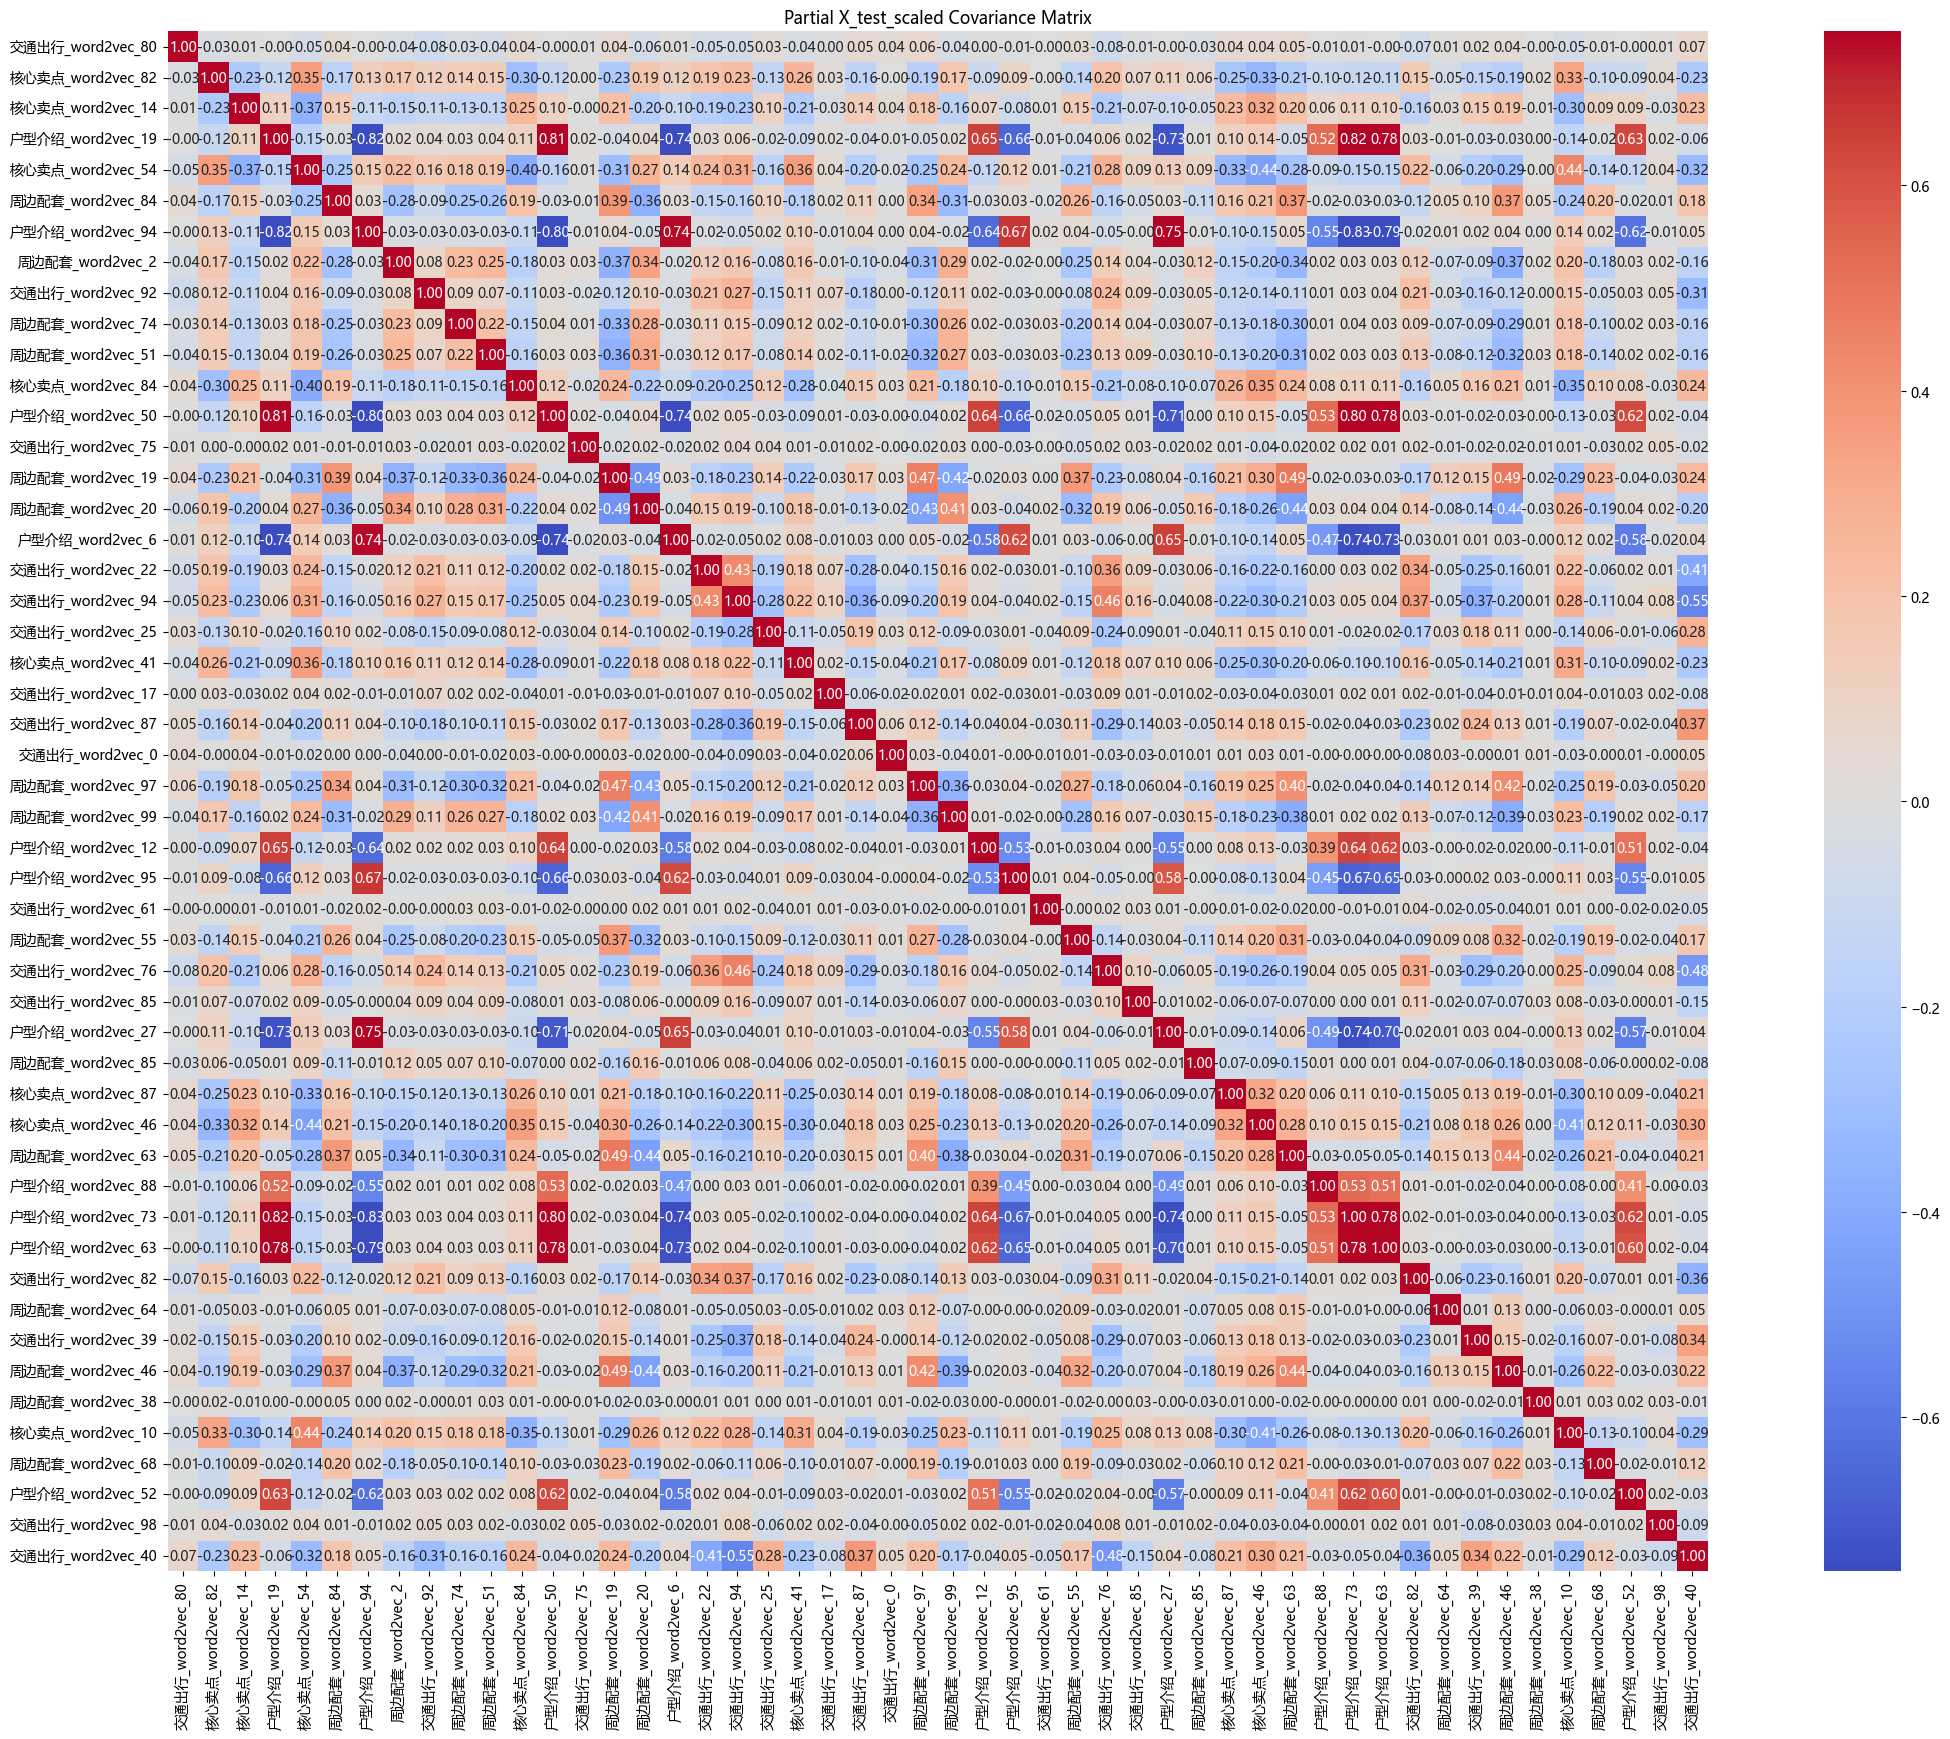
\includegraphics[width=\textwidth]{figures/partial cov martrix test.png}
    \caption{Partial \lstinline|X_test_scaled| Covariance Matrix}
    \label{fig:cov_matrix_plt}
\end{figure}

此外,除了对协方差矩阵进行可视化之外,同时可以画出各变量与目标变量之间的散点图,以直观展示变量之间的相关关系。

\chapter{结语}

第2组在本次房地产估值线性模型中出色的完成了目标任务。我们在深入分析和审计第2组所开发的房地产估值模型后,得出了一系列相对比较丰富的结论和建议。我们的工作不仅涉及了模型的预测能力验证,还包括了对模型稳健性的细致测试,这些都是为了确保模型在实际应用中的可靠性和有效性。通过对模型的全面审计,我们能够识别出潜在的设计缺陷,并提出了相应的修正措施,以避免数据质量问题导致的不良预测结果,即所谓的“Trash in, Trash out”现象。

我们的分析强调了模型验证在提升决策科学性和降低业务风险中的核心作用。通过一系列严格而细致的校验,我们确保了模型的输出预测或决策建议具备高度的可信度。此外,我们将第2组的代码完全剖开透明分析,提高了机器学习决策的透明度和可追溯性,这对于未来在高度监管的行业中建立内外部、前后台之间的信任至关重要。我们提出的模型优化建议旨在通过持续的验证与优化,更好地利用数据的力量,为决策提供坚实的支撑。下面简单回顾我们的一些发现,详细请详细阅读报告。

在数据处理方面,我们发现通过回归分析特定房间数量与建筑面积之间的关系,可以更有效地填补缺失值,而不是简单地使用中位数或固定值。我们还提出了对梯户比例数据进行非线性处理的建议,以及对所在楼层的处理方法,这些都可能对模型的预测精度产生积极影响。

在模型训练与预测部分,我们建议通过交叉验证等方法来评估不同特征选择策略的效果,并选择一个最佳方案。我们还提出了使用递归特征消除(RFE)、基于树的特征选择和基于相关性的特征选择等方法,以优化特征选择过程。

在模型参数调优方面,我们建议使用LassoCV、LassoLarsCV方法直接寻求最优参数,或者通过GridSearchCV、RandomizedSearchCV等方法“搜索”到模型的最优参数组合,以提升模型的预测能力。

最后,我们建议对预测集使用普通最小二乘法(OLS)、Lasso、岭回归(Ridge)和弹性网络(ElasticNet)四种模型进行预测,并提交各自的结果,同时可以通过加权平均的方式得出最终的输出结果,这种方法可能能够提高模型的泛化能力,并减少过拟合的风险。

通过本次审计报告,我们希望能够促进第1组和第2组之间的相互学习和良性竞争,共同推动模型优化和业务发展。我们相信,通过不断的努力和创新,我们可以充分利用数据科学的力量,为房地产估值领域带来更多的突破和进步。


%%%%%%%%%%%%%%%%%%%%%%%%  参考文献  %%%%%%%%%%%%%%%%%%%%%%%%

% \begin{references}
%     \bibliography{references.bib} %指定.bib文件路径
% \end{references}

%%%%%%%%%%%%%%%%%%%%%%%%%  附录  %%%%%%%%%%%%%%%%%%%%%%%%%%

% \StartAppendix % 启用附录

% \chapter{}

% 附录 在这里 

%%%%%%%%%%%%%%%%%%%%%%%  正文后页眉  %%%%%%%%%%%%%%%%%%%%%%

% 页眉(关闭页眉务必将页眉类型设为empty)
\Header
    {common} % 页眉类型:common、publish、empty
    {1pt} % 上分隔线宽度
    {1pt} % 两线距离
    {0.5pt} % 下分割线宽度
    {} % 页眉左自定义内容(文本或图片)
    % {
\includegraphics[width=0.6\textwidth]{figures/logos/school_sf_logo.jpg}} % 页眉中自定义内容(文本或图片)
    {\minorTitleCN}
    {} % 页眉右自定义内容(文本或图片)

%============================================%

% 页脚(关闭页脚务必将页脚类型设为empty) 
\Footer
    {common} % 页脚类型:common、publish、empty
    {0pt} % 上分隔线宽度
    {0pt} % 两线距离
    {0pt} % 下分割线宽度
    {} % 页脚左自定义内容(文本或图片)
    {\thepage} % 页脚中自定义内容(文本或图片)
    {} % 页脚右自定义内容(文本或图片)

%============================================%

% 页数样式 参数:#1起始页数
% \setRomanPageNumber{1} % 设置罗马数字页码
% \setArabicPageNumber{1} % 设置阿拉伯数字页码

%%%%%%%%%%%%%%%%%%%%%%%%%  致谢  %%%%%%%%%%%%%%%%%%%%%%%%%

% \StartAcknowledgements % 启用致谢

% 致谢

\end{document}